%\begin{sidewaysfigure}
%  \begin{center}
%  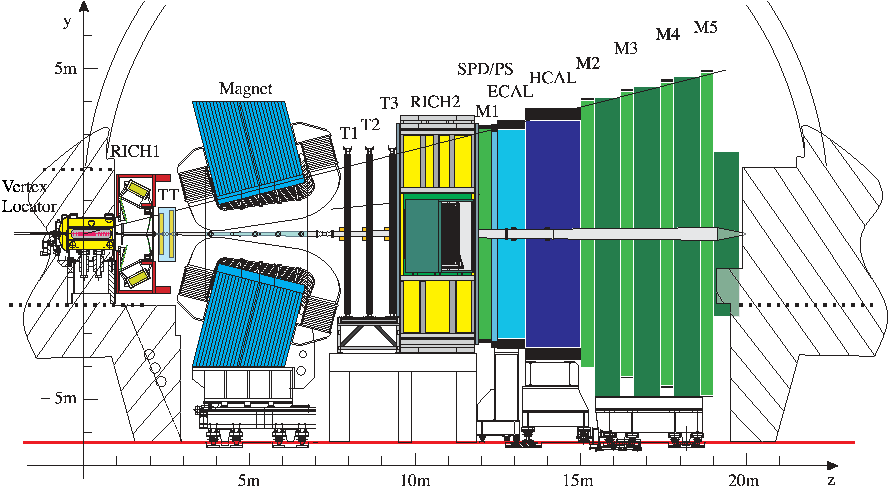
\includegraphics[width=0.8\textheight]{lhcb-detector-cross-section}
%  \caption[Cross-section view of \LHCb, cut in the non-bending $y$--$z$ plane]%
%    {Cross-section view of \LHCb, cut in the non-bending $y$--$z$ plane.}
%  \label{fig:LHCbCrossSection}
%  \end{center}
%\end{sidewaysfigure}



\chapter{Enhanced ECal reconstruction}
\label{chap:EnhancedECalReconstruction}
The current implementation of the ECal reconstruction software was designed to reconstruct particles which originate from the ND280 tracker and enter the ECal.  As section~\ref{sec:ECalEventReconstruction} shows, this was realised by only considering ECal hit clusters under the single track-like or shower-like hypothesis.  It should be evident that a neutrino interaction occurring within the ECal does not well fit this topology.  While it is true that there is some power in the current reconstruction to distinguish a neutrino interaction from an entering track or shower, there is little feature information available.  How many final state particles propagated from the interaction?  How much visible energy was deposited by each of the particles?  Where in the ECal did the interaction occur?  These basic questions can not be trivially answered when using the current reconstruction.  To maximise the ability of distinguishing ECal neutrino interactions from entering backgrounds, the reconstruction must be revisited.

\section{The Hough transform}
\label{sec:HoughTransform}
The Hough transform is a popular method of machine pattern recognition used by, but is not limited to, high energy physics experiments.  Originally designed for machine track recognition in bubble chamber pictures~\cite{Hough:1959qva}, the version most widely used throughout the world was developed in 1972~\cite{Duda:1972:UHT:361237.361242}.  The Hough transform is used to isolate specific features or shapes from a digital image.  The simplest implementation, which is of most interest in event reconstruction, allows the extraction of straight, 2D lines from a complex pattern.  This is acheived by exploitation of a very simple feature of 2D geometry.

\subsection{Line-point duality}
\label{subsec:LinePointDuality}
Consider a straight line formed in a 2D cartesian space as shown in Fig.~\ref{fig:2DCartesianLine}.  The line is usually described by
\begin{equation}
  y = mx + c
  \label{eq:2DLineCartesean}
\end{equation}
where $y$ and $x$ are used as coordinates, $m$ is the gradient of the line and $c$ is the intercept location of the line with the $y$ axis.  While it is not necessary to analyse this simple shape in great detail, it is important to note that $m$ and $c$ are the only parameters necessary to completely describe the line.  
\newline
Now consider a new 2D space where the axes are defined by $m$ and $c$ rather than $x$ and $y$ (here after referred to as the parameter space).  As this parameter space is described by the parameters of a general 2D cartesian line, there is an underlying symmetry between the two spaces.  The parameters of the 2D line shown in Fig.~\ref{fig:2DCartesianLine} can be used to form a pair of coordinates ($m$,$c$) in the parameter space as shown in Fig.~\ref{fig:2DParameterPoint}.  It is important here to state clearly the general result; a straight line in cartesian space is represented by a single point in parameter space. 
\begin{figure}
  \centering
  \parbox{7cm}{
    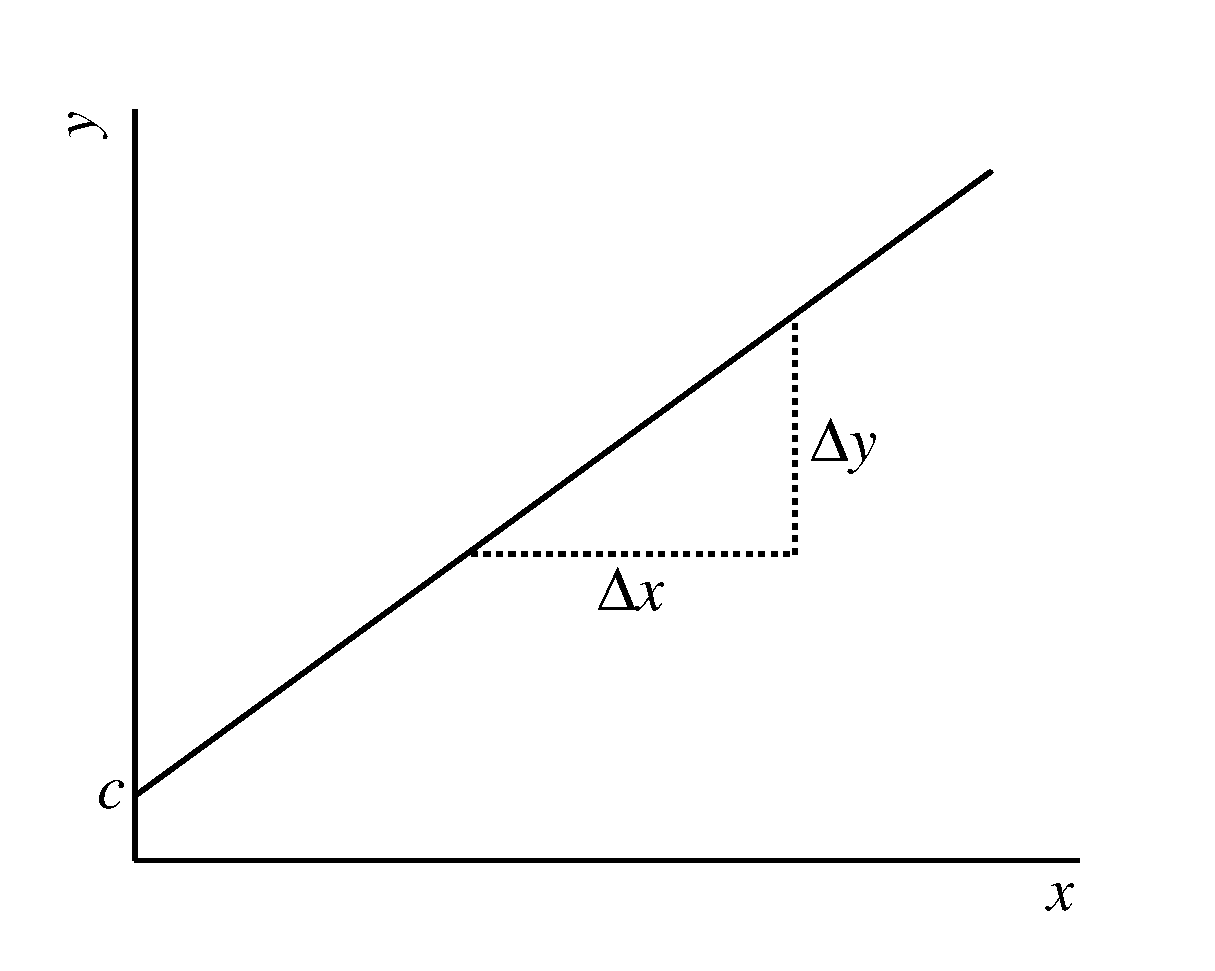
\includegraphics[width=7cm]{images/hough_transform/cartesian_line}
    \caption{Line in 2D cartesian space.}
    \label{fig:2DCartesianLine}}
    \qquad
    \begin{minipage}{7cm}
      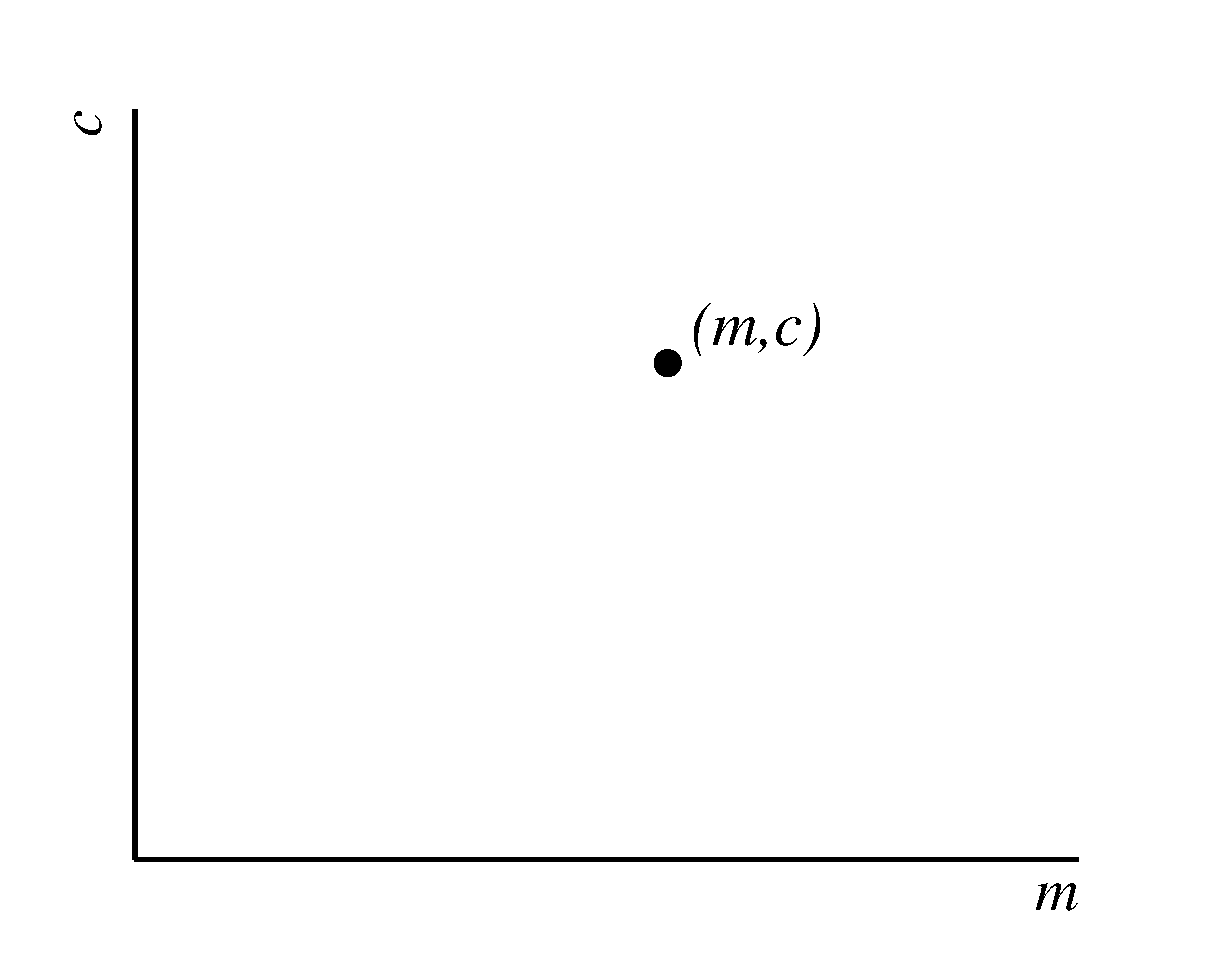
\includegraphics[width=7cm]{images/hough_transform/parameter_point}
      \caption{Point in 2D parameter space.}
      \label{fig:2DParameterPoint}
    \end{minipage}
\end{figure}
\newline
Now consider the 2D cartesian space again.  Unlike before, we will define a single point rather than a straight line. Such a point is traditionally described by a pair of coordinates ($x$,$y$).  However, an alternative description of the point is an infinite number of lines all of which pass through ($x$,$y$).  This is highlighted by Fig.~\ref{fig:2DCartesianPoint} where three lines of the infinite set are shown along with the point they represent.  As the infinite line set are used to describe a single point, all lines in the set must follow a pattern.  This relationship is revealed by simple algebraic manipulation of equation~\ref{eq:2DLineCartesean} to give
\begin{equation}
  c = -xm + y.
  \label{eq:2DLineParameter}
\end{equation}
Despite the manipulation, equation~\ref{eq:2DLineParameter} still resembles the equation of a 2D line, however the parameters are $x$ and $y$ and the coordinates are $m$ and $c$.  Specifically, equation~\ref{eq:2DLineParameter} is represented by a line in the parameter space defined above.  The gradient of this line is 
\begin{equation}
  x = \frac{\Delta c}{\Delta m}
  \label{eq:2DLineGradientParameterSpace}
\end{equation}
and the intercept of the line with the $c$ axis is $y$ as shown in Fig.~\ref{fig:2DParameterLine}.  As before, it is important to clearly state what has been shown; a point in cartesian space is represented by a line in parameter space.

\begin{figure}
  \centering
  \parbox{7cm}{
    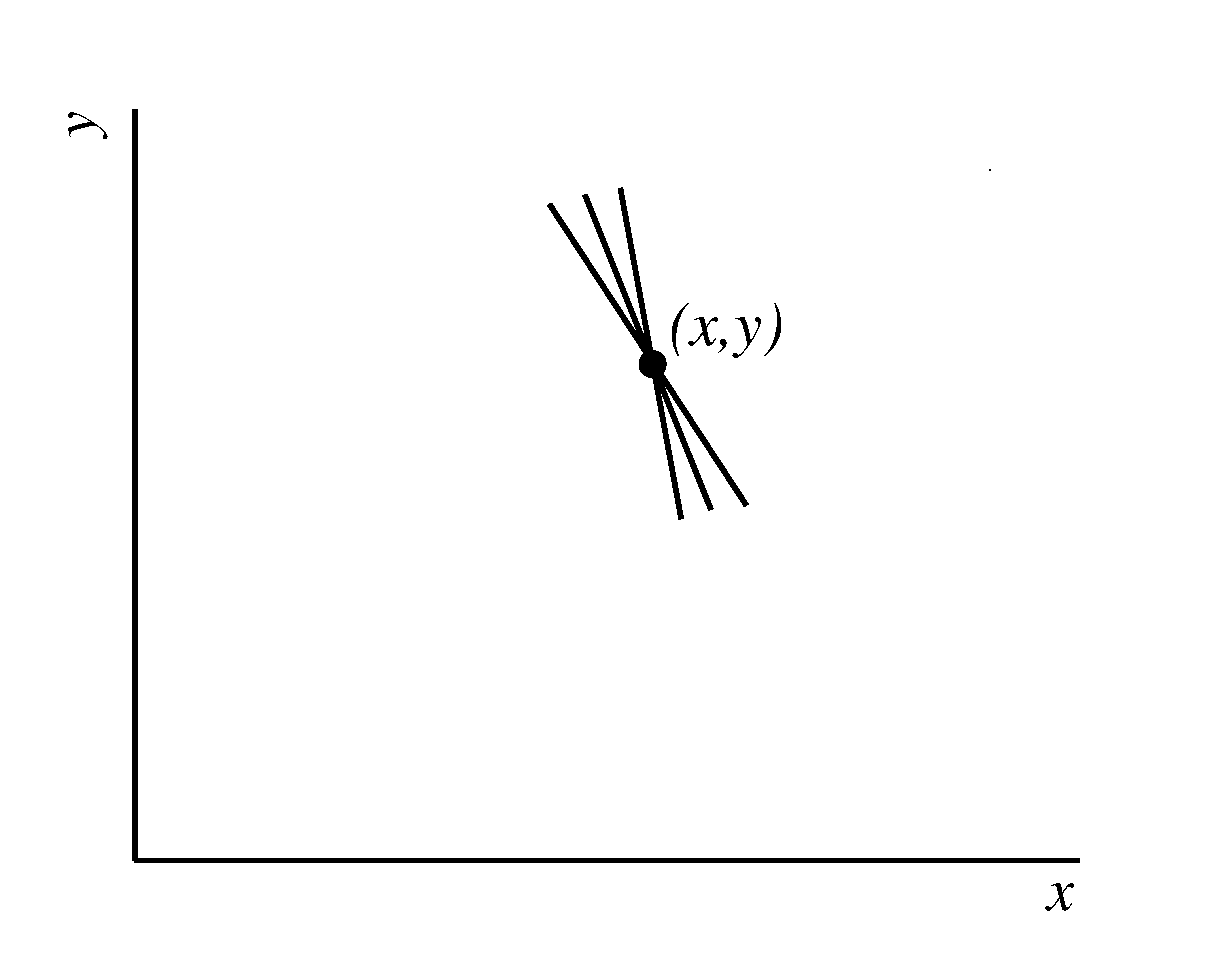
\includegraphics[width=7cm]{images/hough_transform/cartesian_point}
    \caption{Point in 2D cartesian space.}
    \label{fig:2DCartesianPoint}}
    \qquad
    \begin{minipage}{7cm}
      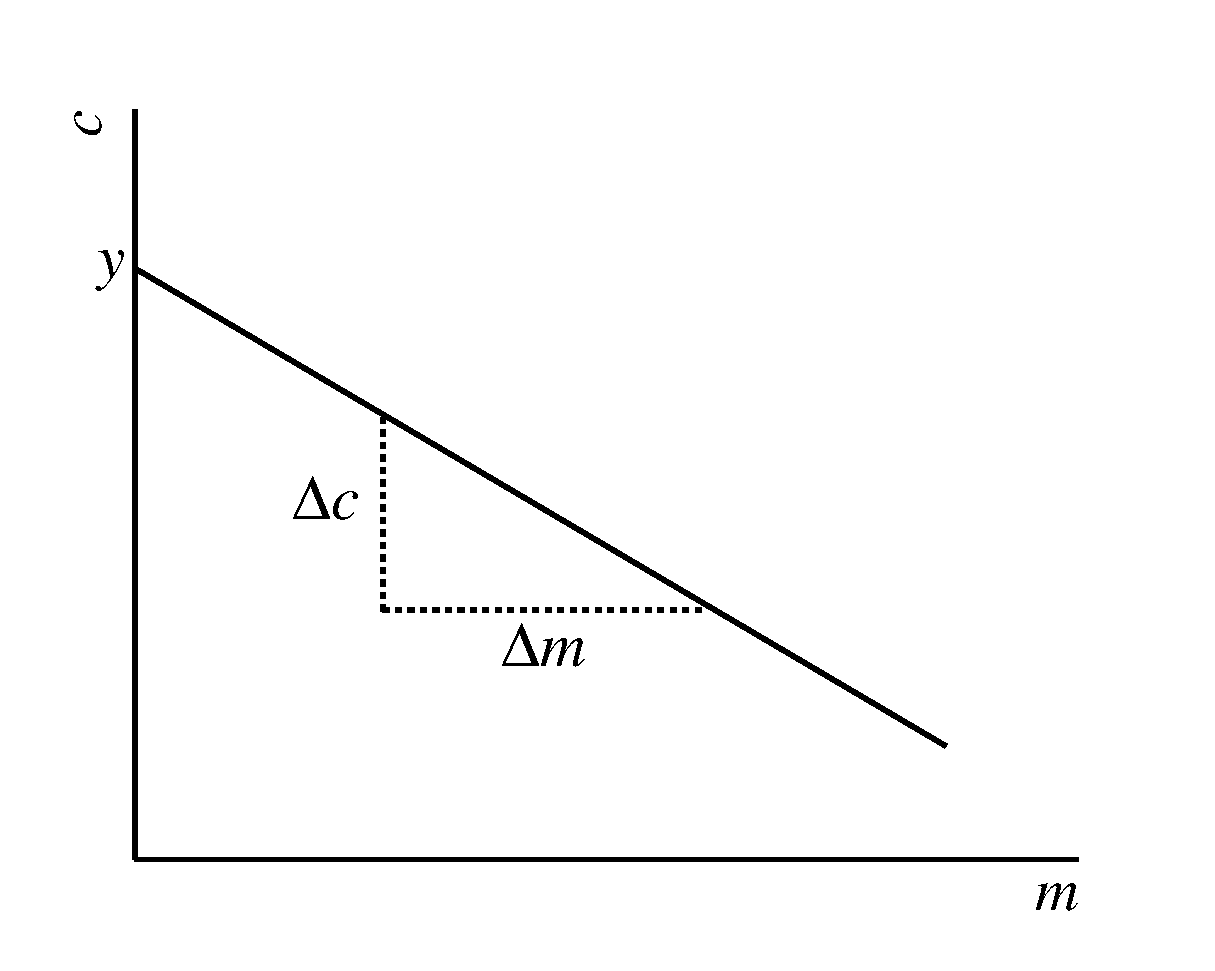
\includegraphics[width=7cm]{images/hough_transform/parameter_line}
      \caption{Line in 2D parameter space.}
      \label{fig:2DParameterLine}
    \end{minipage}
\end{figure}

\subsection{The parameter space}
\label{subsec:ParameterSpace}
As section~\ref{subsec:LinePointDuality} shows, there is a clear relationship between the cartesian space and the parameter space.  Specifically, there is a symmetry between lines and points in the two spaces.  This relationship between the cartesian and parameter spaces is not only interesting but also very powerful.  Consider again the parameter line defined by equation~\ref{eq:2DLineParameter} and shown in Fig.~\ref{fig:2DParameterLine}.  As shown in section~\ref{subsec:LinePointDuality}, equation~\ref{eq:2DLineParameter} was derived by considering the infinite set of lines which pass through a cartesian point.  As this infinite set represents the parameter line, it must also be true that the parameter line represents the infinite line set.  Using one of the results from section~\ref{subsec:LinePointDuality}, any point along the parameter line represents one of the lines from our infinite set.  This key feature of the parameter space is the central component of the Hough transform.  
\newline
We will now return to the cartesian space for an example of how the Hough transform works.  Let's define three points in this space,
\begin{equation}
  \begin{split}
    &\quad p_{1}: (2,6) \\
    &\quad p_{2}: (4,8) \\
    &\quad p_{3}: (6,10).
  \end{split}
  \label{eq:HTExampleCartesianPoints}
\end{equation}

\begin{figure}
  \centering
  \parbox{7cm}{
    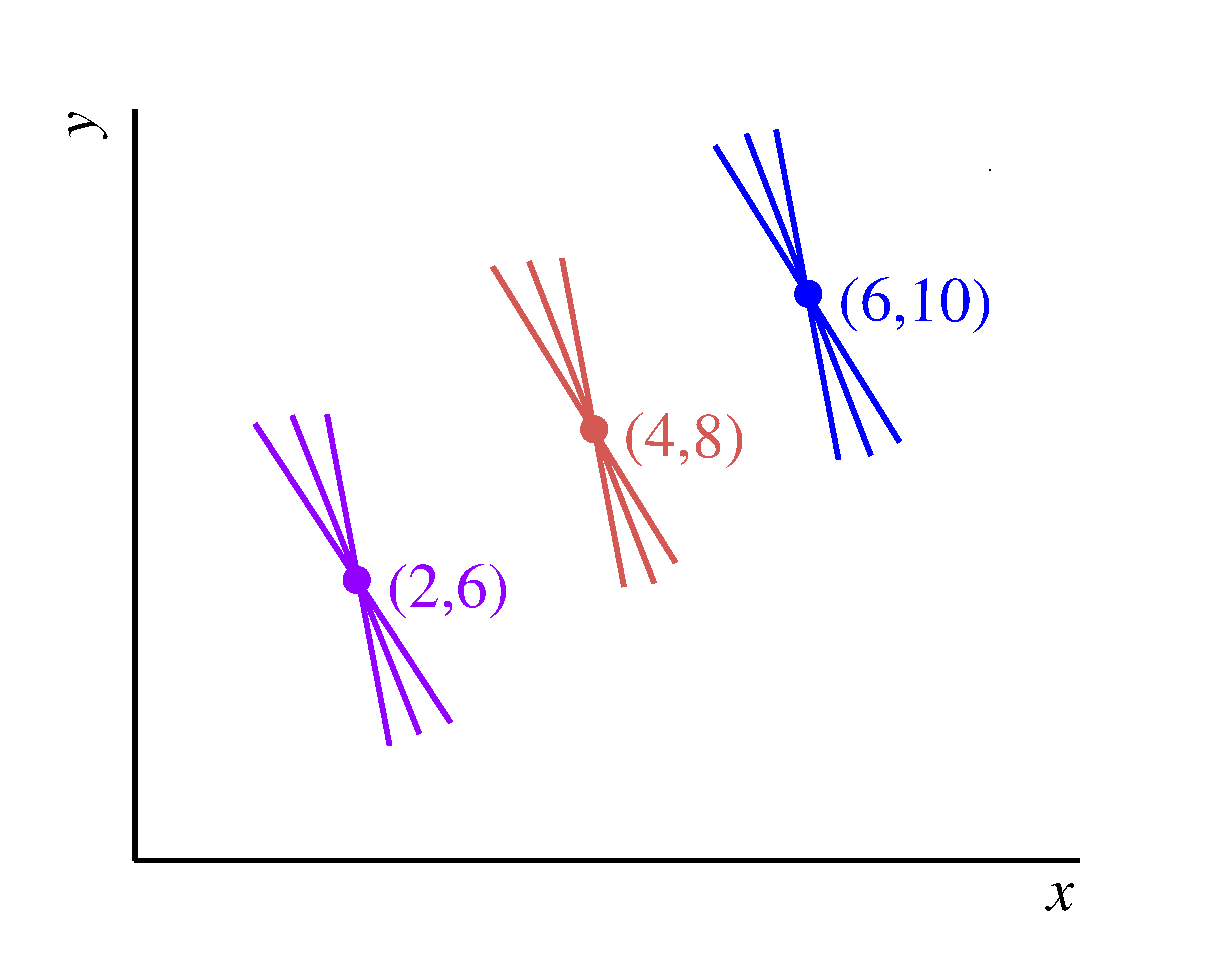
\includegraphics[width=7cm]{images/hough_transform/HT_example_cartesian_space}
    \caption{The three cartesian points defined in equation~\ref{eq:HTExampleCartesianPoints}.  The colour coding matches that of Fig.~\ref{fig:HTExampleParameterSpace}.}
    \label{fig:HTExampleCartesianSpace}}
    \qquad
    \begin{minipage}{7cm}
      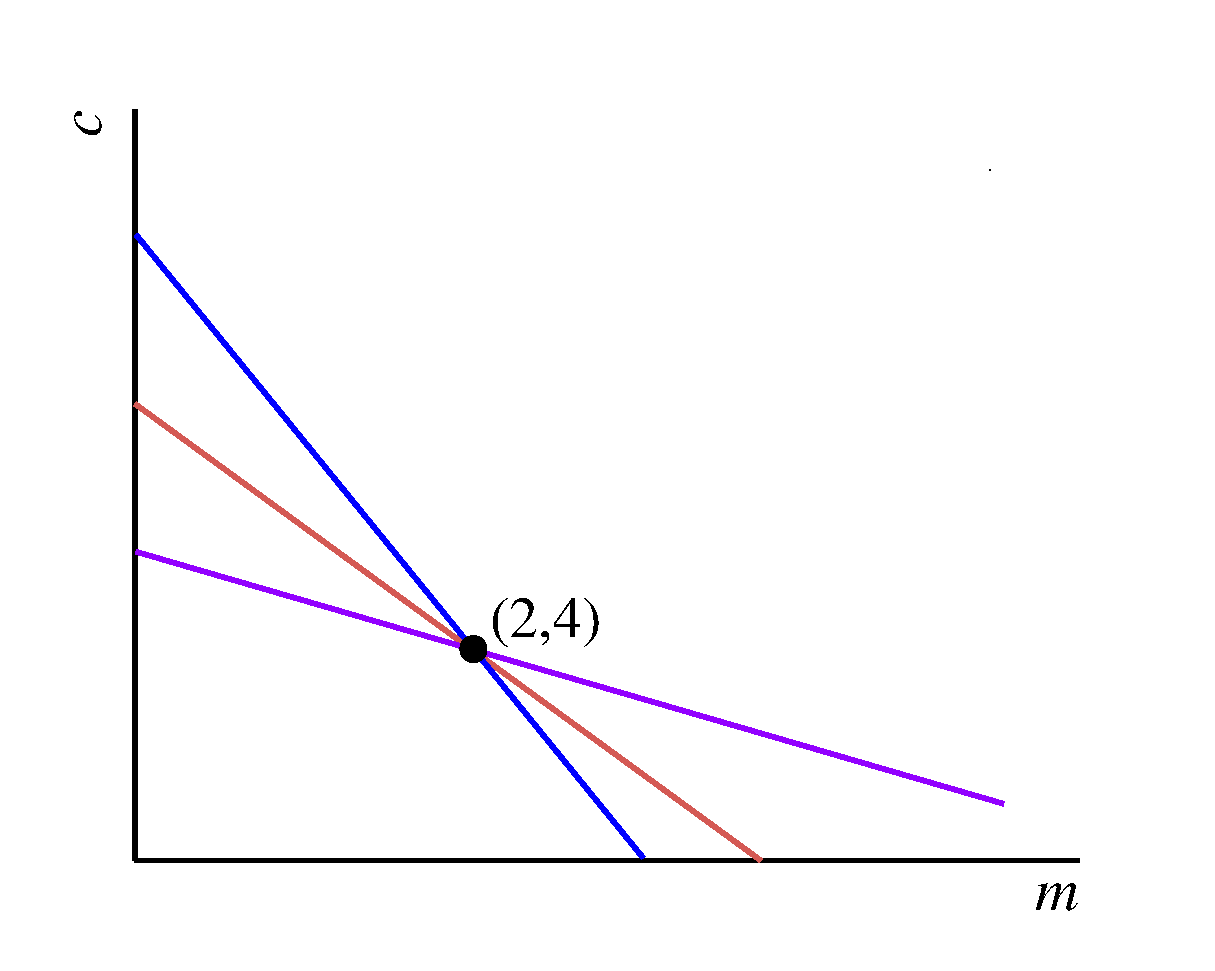
\includegraphics[width=7cm]{images/hough_transform/HT_example_parameter_space}
      \caption{The three parameter lines defined in equation~\ref{eq:HTExampleParameterLines}.  The same colour coding as Fig.~\ref{fig:HTExampleCartesianSpace} is used.}
      \label{fig:HTExampleParameterSpace}
    \end{minipage}
\end{figure}
The three points defined in equation~\ref{eq:HTExampleCartesianPoints} are shown in Fig.~\ref{fig:HTExampleCartesianSpace}.  Using one of the results from section~\ref{subsec:LinePointDuality} and equation~\ref{eq:2DLineParameter}, the three points can be Hough transformed into the following parameter lines:
\begin{equation}
  \begin{split}
    &\quad c = -2m + 6 \\
    &\quad c = -4m + 8 \\
    &\quad c = -6m + 10.
  \end{split}
  \label{eq:HTExampleParameterLines}
\end{equation}
The three parameter lines are shown in Fig.~\ref{fig:HTExampleParameterSpace}.  From Fig.~\ref{fig:HTExampleParameterSpace}, it is clear that the three parameter lines all cross at a common point with parameter space coordinates (2,4).  Using the results from section~\ref{subsec:LinePointDuality}, this common point in parameter space is represented by a line in cartesian space.  In addition, as (2,4) is common to all three parameter lines, the cartesian line represented by (2,4) must also pass through all three cartesian points defined by equation ~\ref{eq:HTExampleCartesianPoints}.  This new cartesian line is defined by
\begin{equation}
  y = 2x + 4
  \label{eq:HTExampleCartesianLine}
\end{equation}
and is shown in Fig.~\ref{fig:HTExampleCartesianSpaceWithLine} with the original points used to generate the parameter lines.  While this example is relatively simple, it demonstrates the capability of the Hough transform to recognise linear patterns in sets of points.

\begin{figure}
  \centering
  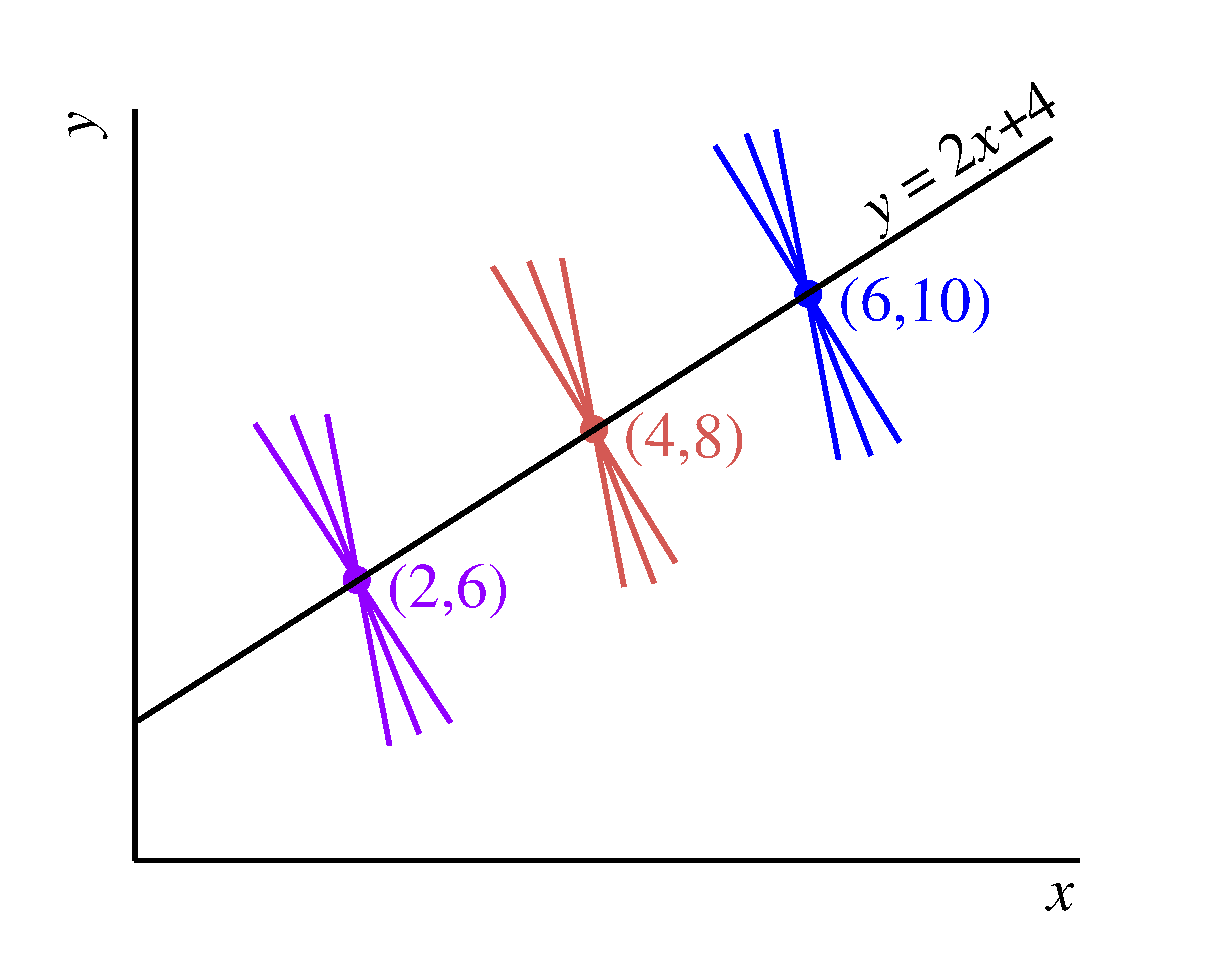
\includegraphics[width=9cm]{images/hough_transform/HT_example_cartesian_space_with_line}
  \caption{The line represented by the intersection in Fig.~\ref{fig:HTExampleParameterSpace} with the cartesian points it intercepts.}
  \label{fig:HTExampleCartesianSpaceWithLine}
\end{figure}

\subsection{Redefinition of parameters}
\label{subsec:ParameterRedefinition}
Unfortunately, a complication in computation arises when $m\rightarrow\infty$.  However, this complication can be removed by redefining the line parameters such that one is bounded.  An alternative 2D line parameterisation is to specify a line in terms of the angle it makes with the $x$ axis, $\theta$, and the perpendicular distance of the line from the origin, $\rho$, as illustrated in Fig.~\ref{fig:CartesianParameterRedefinition}.  The functional form of the cartesian line becomes 
\begin{equation}
  y = x\textrm{tan}\theta + \frac{\rho}{\textrm{cos}\theta}.
  \label{eq:CartesianLineReparameterisation}
\end{equation}
Using this new parameterisation, we must also define a new parameter space with axes $\theta$ and $\rho$.  Using equation~\ref{eq:CartesianLineReparameterisation}, a line in this new parameter space is defined by
\begin{equation}
  \rho = y\textrm{cos}\theta - x\textrm{sin}\theta.
  \label{eq:ParameterLineReparameterisation}
\end{equation}
By definition, the $\theta$ axis of the parameter space must be bounded to the interval [0,2$\pi$].  If the directionality of the line is meaningless to the analyser, then the interval can be restricted to [0,$\textrm{\pi}$].
\newline
The disadvantage of this parameterisation is that parameter line generation now involves trigonometric calculations which can be computationally expensive.  However, this problem is small when compared to the unbounded complication of the traditional parameterisation.

\begin{figure}
  \centering
  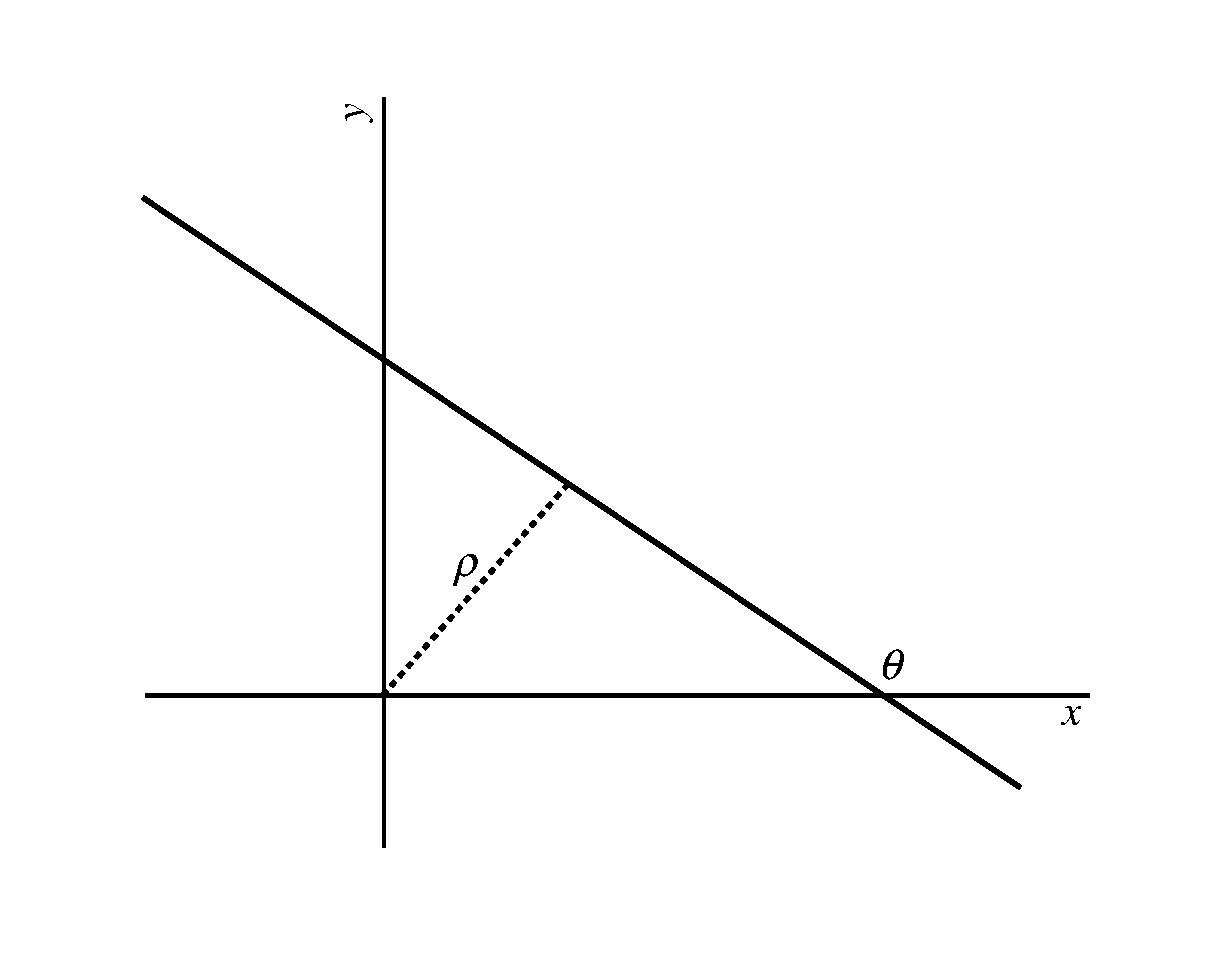
\includegraphics[width=9cm]{images/hough_transform/cartesian_parameter_redefinition}
  \caption{$\theta-\rho$ parameterisation of a 2D line.}
  \label{fig:CartesianParameterRedefinition}
\end{figure}



\subsection{Discretisation of the parameter space}
\label{subsec:ParameterSpaceDiscretisation}
It must now be considered how the parameter space is analysed.  When a large number of parameter lines are generated, it becomes computationally expensive to analyse the resultant parameter space.  While approaches exist to analyse the parameter space with very high precision~\cite{331821}, it is often only necessary to extract parameters with finite resolution.  In such a case, it is convenient to discretise the parameter space.  Under this regime, the parameter space is split into $\theta-\rho$ bins.  Then, a parameter line is generated by incrementing the value of each $\theta-\rho$ bin it passes through.  After each line has been added to the parameter space, the crossing locations can be readily found by searching for the $\theta-\rho$ bins with content larger than unity.  An example of this discretisation is illustrated in Fig.~\ref{fig:BinnedParameterSpace}, where the parameter lines defined in equation~\ref{eq:HTExampleParameterLines} have be re-parameterised using equation~\ref{eq:ParameterLineReparameterisation} and plotted.  The content of each bin in Fig.~\ref{fig:BinnedParameterSpace} records how many of the three parameter lines pass through each bin.  The bin with value 3 is the crossing point of the three parameter lines.
\newline
If a discretised approach is acceptable, which is the case in event reconstruction, construction and analysis of the parameter space is reduced to filling a 1D array $N$ times, where $N$ is the number of parameter lines, followed by a 1D grid search of the array to find the bin with the highest content.
\begin{figure}
  \centering
  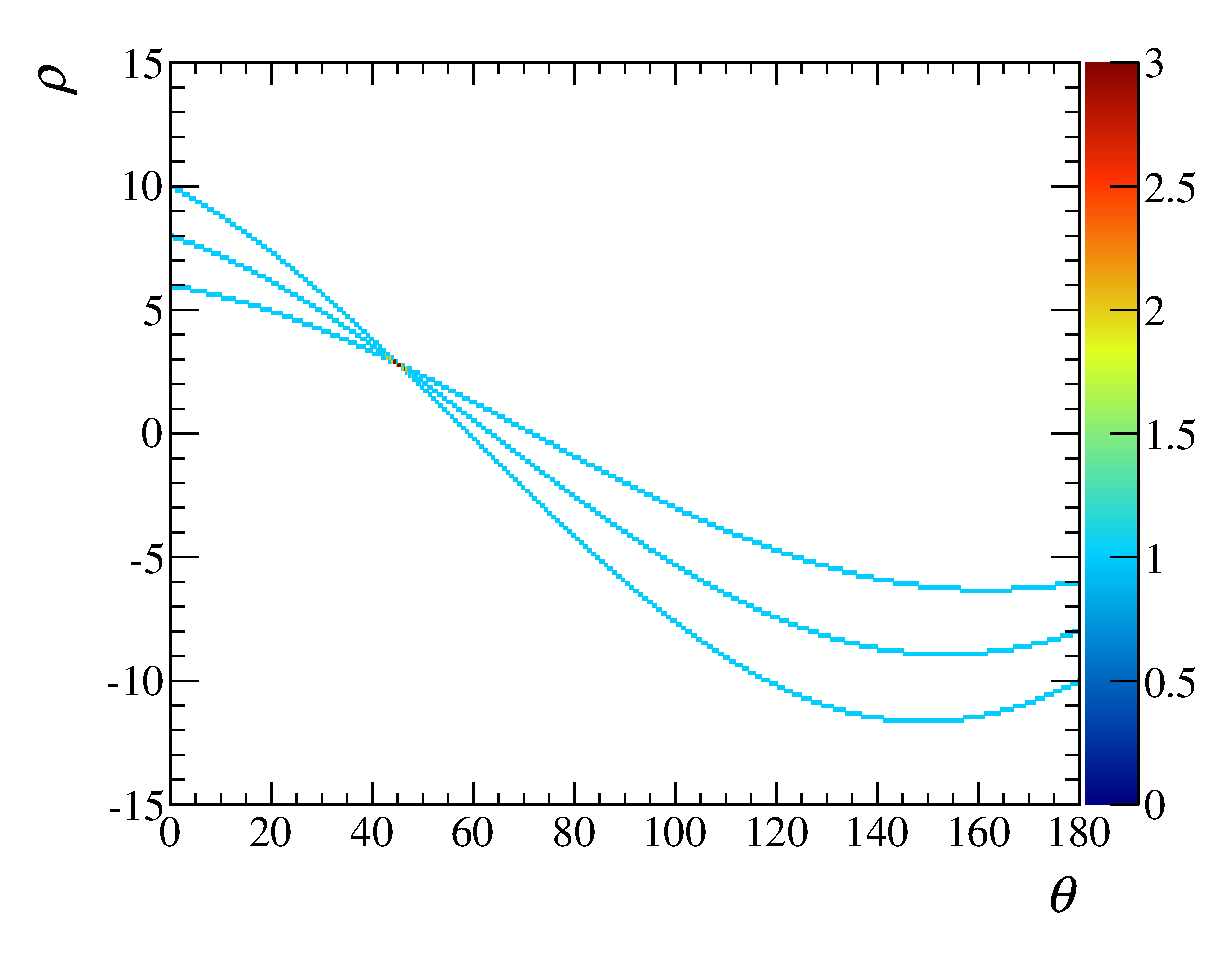
\includegraphics[width=9cm]{images/hough_transform/binned_parameter_space}
  \caption{The discrete $\theta-\rho$ space.  The plotted lines are those defined in equation~\ref{eq:HTExampleParameterLines} and reparameterised using equation~\ref{eq:ParameterLineReparameterisation}.}
  \label{fig:BinnedParameterSpace}
\end{figure}



\section{ECal application of the Hough transform}
\label{sec:ECalApplicationHoughTransform}
We must now address how the Hough transform can be used as a reconstruction tool in the ECal.  To do this, let's consider a neutrino interaction which occurs in the ECal as illustrated in~\ref{fig:3StateInteractionNoReconstruction}.  While the propagating neutrino is invisible to the ECal, the charged final state are definitely not.  To first order, the final state particles propagate in straight lines depositing energy in the scintillator bars as they go.  From this, we can infer that the hit bars arranged in straight lines should reveal the trajectory of the final states.  As shown above, the Hough transform is capable of identifying straight lines from a set of coordinates.  However, there are two complications in the ECal which the above sections have not addressed.  We have only specifically discussed how to extract a single straight line from a pattern.  As Fig.~\ref{fig:3StateInteractionNoReconstruction} shows, the number of final states can be, and is often, greater than one.  This is merely a problem of computation which will be addressed in section~\ref{subsec:ParameterSpaceAnalysis}.  A much more severe problem is that the above demonstrations only deal with patterns constructed from infinitesimal points.  While the centre of a scintillator bar can be used as a point for parameter line generation, it is unlikely that a final state particle will pass through the central point of the scintillator bars that it propagates through.  If this is not addressed, the Hough transform will be of little use in trajectory reconstruction.
\begin{figure}
  \centering
  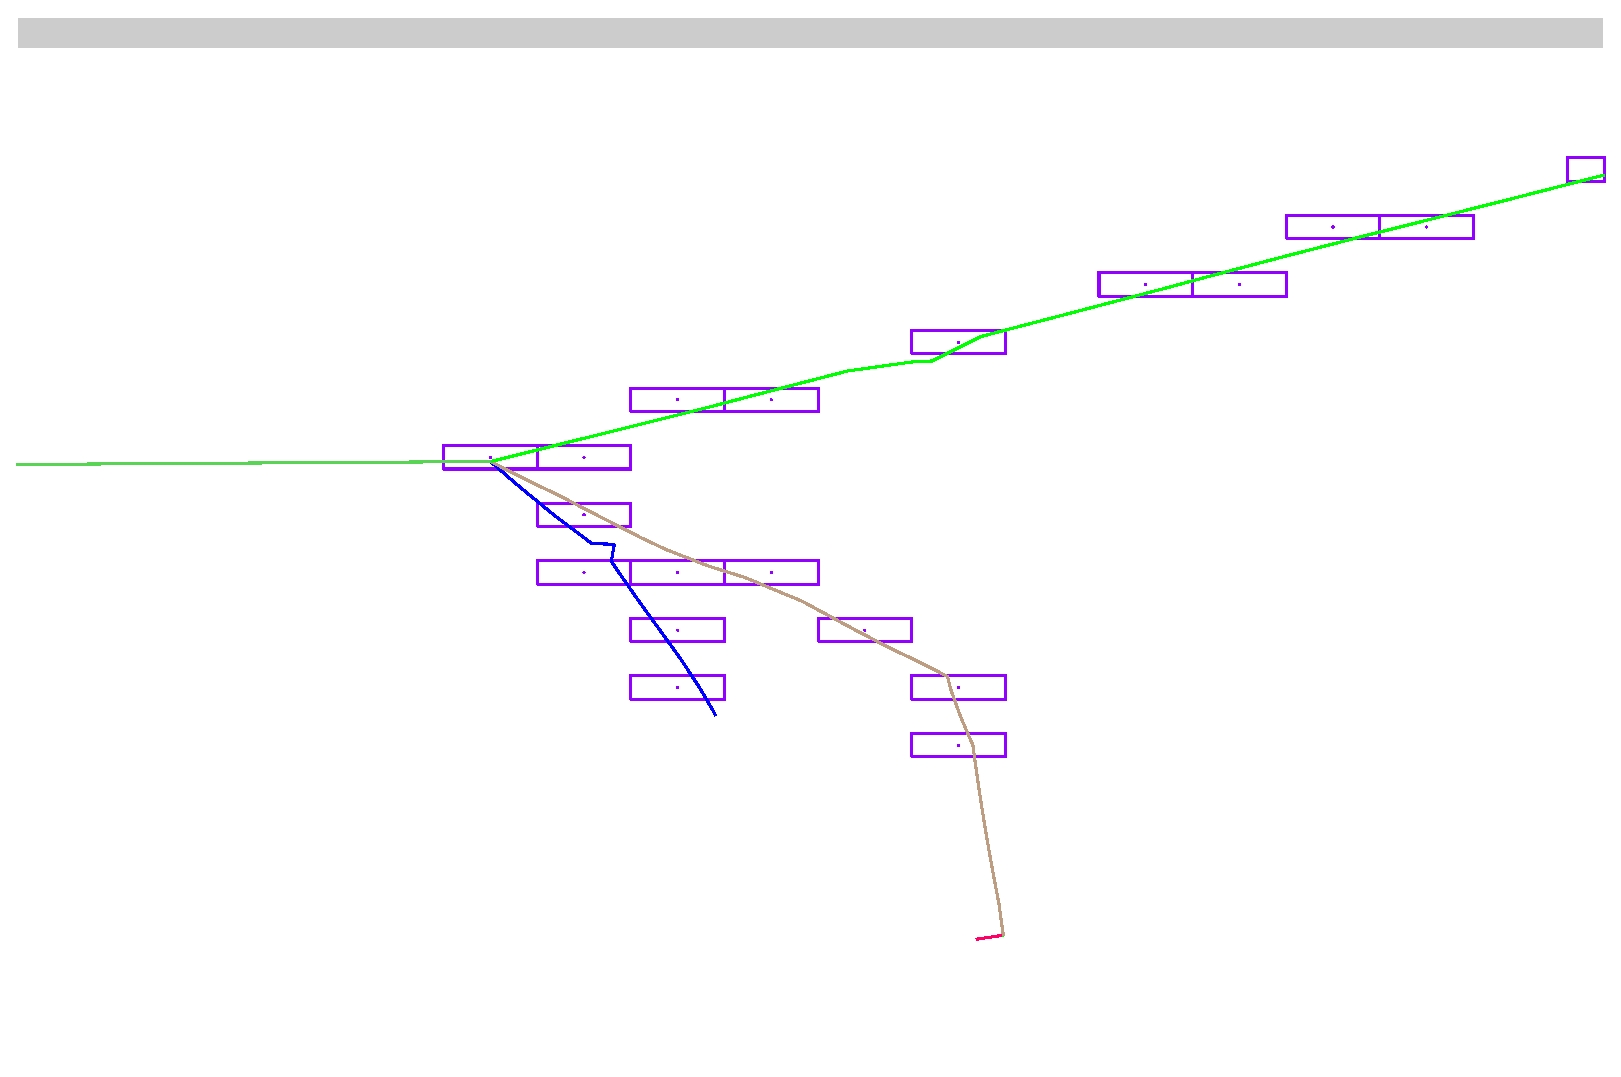
\includegraphics[width=10cm]{images/hough_transform/3StateInteraction_SideLeftECal_NoReconstruction.eps}
  \caption{Simulated neutrino interaction with 3 final states in the side-right ECal.  The green line entering from the left is the $\nu_\mu$.  The green line exiting to the right is a $\mu^{-}$, the brown line is a $\pi^+$ and the blue line is a proton.  The purple rectangles represent the hit ECal bars.}
  \label{fig:3StateInteractionNoReconstruction}
\end{figure}

\subsection{Modelling the ECal bar}
\label{subsec:ECalBarModel}
To make the Hough transform viable as a reconstruction tool, the finite dimensions of the ECal bar need to be incorporated into the parameter space generation.  This feature of the ECal bars would be very problematic if the parameter space was continous.  However, it is only necessary to know the line parameters with finite resolution and a discrete parameter space can be used.  This means that the ECal bar can be modelled as a set of cartesian points and each of said points can be Hough transformed in turn to build up the parameter line representation of the ECal bar.
\newline
There are now two steps to consider.  Firstly, how should the points be arranged?  Remember that the Hough transform of a point represents all of the lines that pass through that point.  So, the points should be arranged in such a fashion that any line which passes through the 2D cross-section of the ECal bar also has to pass through one of the points in the configuration.  Secondly, the spacings between the points should be small enough that no gaps appear in the generated parameter line.  
\newline
Assuming that every bin of the parameter space will have a 1$^\circ\times$1 mm area, an obvious choice would be to use a rectangular grid of points with 1 mm spacing superimposed over the 2D cross-section of an ECal bar.  The total number of points used to model the ECal bar is 451.  To Hough transform the ECal bar, every point in the grid array can be Hough transformed individually with care taken to ensure that each $\theta-\rho$ bin is filled exactly once.  The result is illustrated in Fig.~\ref{fig:ECalBarHoughTransformGridRepresentation}.  The finite size of the ECal bar is evident by the finite size of the resultant parameter line.
\begin{figure}
  \centering
  \parbox{7cm}{
    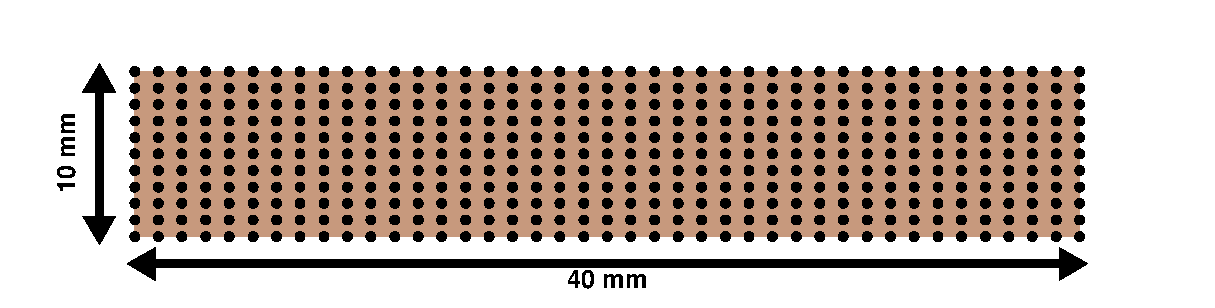
\includegraphics[width=7cm]{images/ecal_hough_transform/ecal_grid_array.eps}
    \caption{Grid representation of an ECal bar.}
    \label{fig:ECalBarGridRepresentation}}
    \qquad
    \begin{minipage}{7cm}
      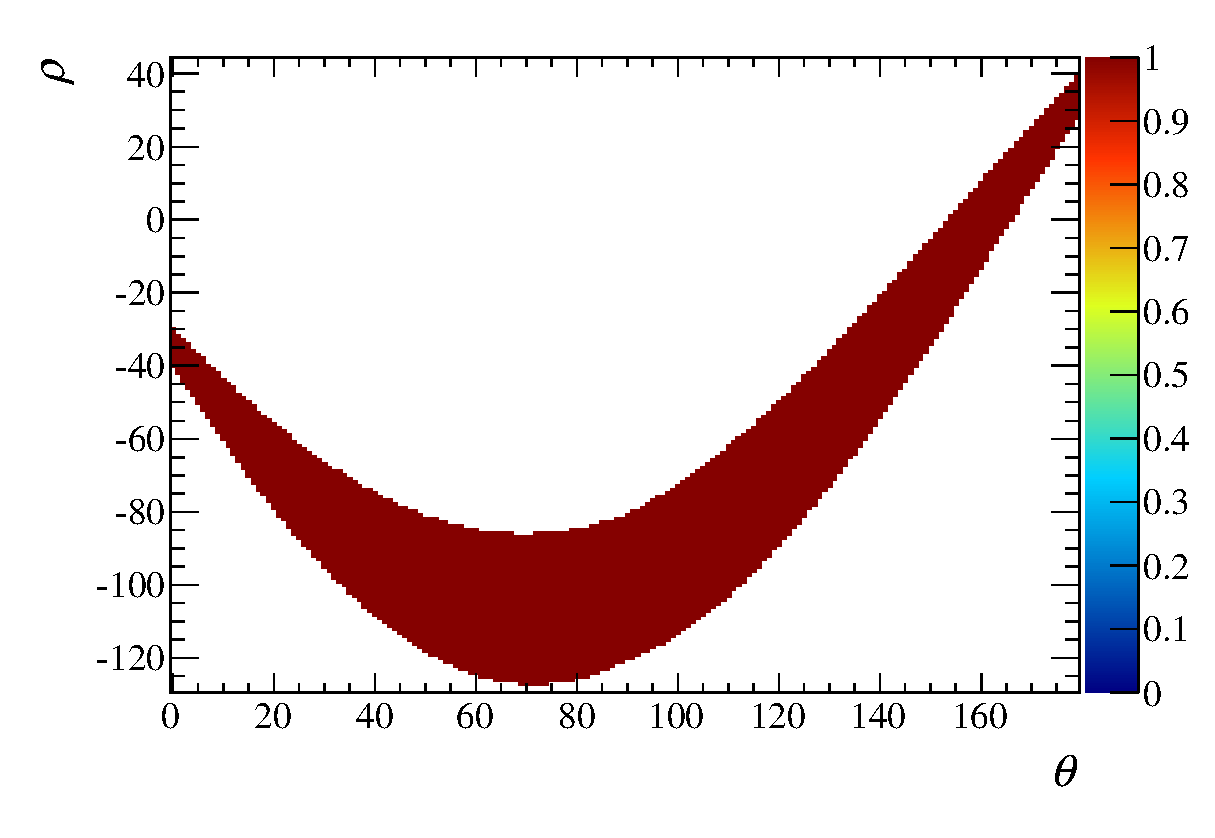
\includegraphics[width=7cm]{images/ecal_hough_transform/single_ecal_bar_hough_transform.eps}
      \caption{Single ECal bar Hough transform using the point configuration shown in Fig.~\ref{fig:ECalBarGridRepresentation}.}
      \label{fig:ECalBarHoughTransformGridRepresentation}
    \end{minipage}
\end{figure}
\newline
While the generated parameter line accurately represents every line which passes through the ECal bar, there are two problems with this approach.  Firstly, the large number of points to be Hough transformed is very large which results in a long CPU time.  Secondly, there is a very high number of redundant calculations involved in the parameter line generation.  Consider an exactly vertical line which passes through one of the points in the grid array.  This line also passes through 10 other points in the same column of the grid.  This means that when the parameter line is being generated, this vertical line is calculated 11 times for each column.  Bearing this in mind, there are many points along the parameter line which are repeatedly calculated and provide no extra information.  This would mean that any algorithm which uses this approach would be very CPU inefficient.
\newline
An alternative is to model the ECal bar as a set of points arranged in a cross as shown in Fig.~\ref{fig:ECalBarCrossRepresentation}.  Assuming that the spacing bettween the points on each line of the cross is infinitesimal, any line which passes through the ECal bar would also have to pass through one of the points in the configuration.  As the parameter space is discrete, the spacing between the points need to be infinitesimal but only small enough to ensure that no gaps appear in the parameter line.  Using 45 points on each line of the cross, the ECal bar can be Hough transformed by Hough transforming each point in the cross. An example of this result is shown in Fig.~\ref{fig:ECalBarHoughTransformCrossRepresentation} using the same ECal bar used to generate Fig.~\ref{fig:ECalBarHoughTransformGridRepresentation}.  Clearly, Fig.~\ref{fig:ECalBarHoughTransformGridRepresentation} and Fig.~\ref{fig:ECalBarHoughTransformCrossRepresentation} are identical showing that the cross model achieves the same result as the grid model.  Comparing the two, the cross model uses a 90 point representation whereas the grid model uses a 451 point representation.  This should mean that an algorithm utilising the cross model would be a factor of five faster than one using a grid model.  In addition to this, the number of redundant calculations is heavily reduced.
\begin{figure}
  \centering
  \parbox{7cm}{
    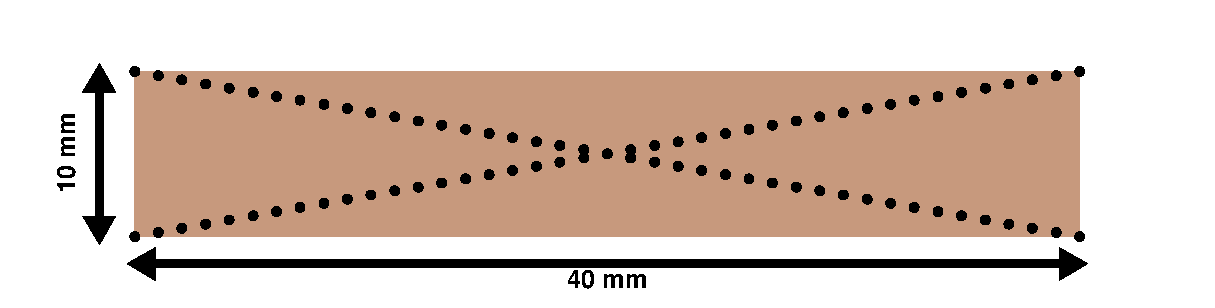
\includegraphics[width=7cm]{images/ecal_hough_transform/ecal_cross_array.eps}
    \caption{Cross representation of an ECal bar.}
    \label{fig:ECalBarCrossRepresentation}}
    \qquad
    \begin{minipage}{7cm}
      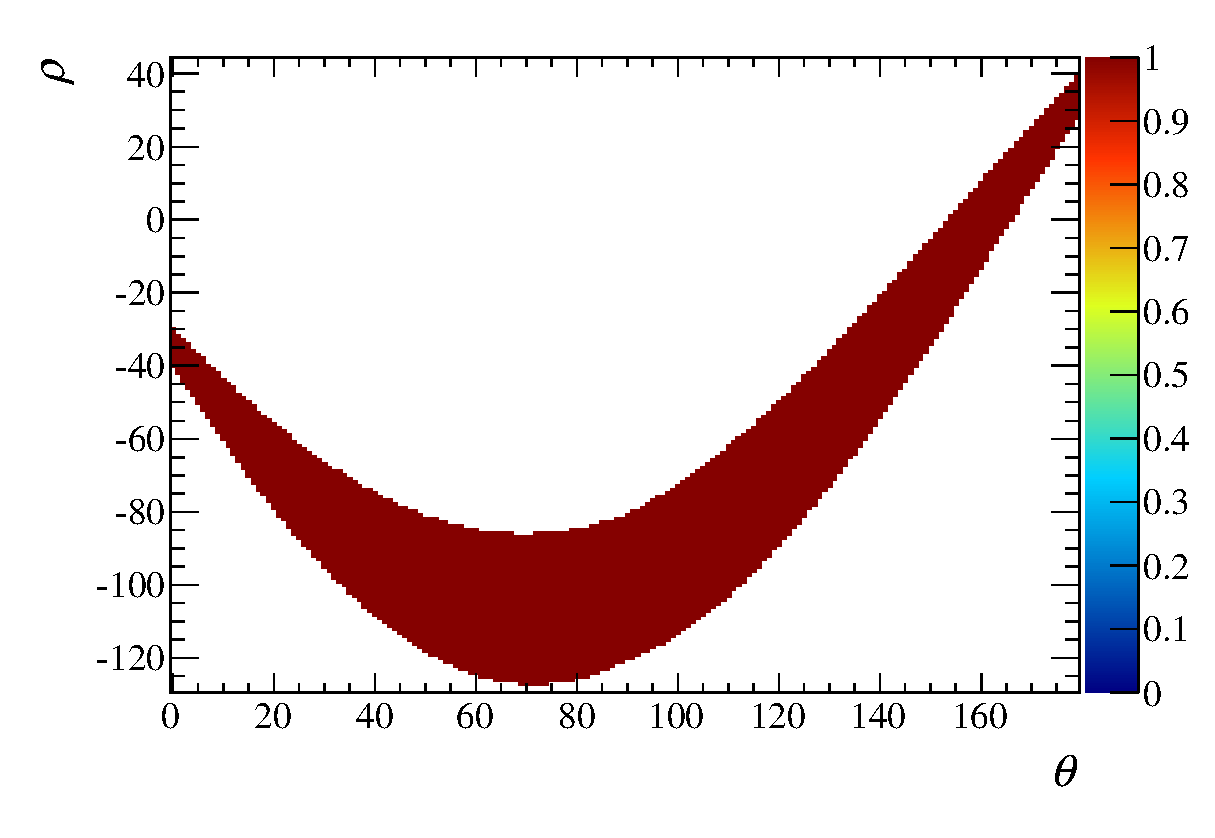
\includegraphics[width=7cm]{images/ecal_hough_transform/single_ecal_bar_hough_transform.eps}
      \caption{Single ECal bar Hough transform using the point configuration shown in Fig.~\ref{fig:ECalBarCrossRepresentation}.}
      \label{fig:ECalBarHoughTransformCrossRepresentation}
    \end{minipage}
\end{figure}
%\subsection{ECal bar Hough transform}
%\label{subsec:ECalBarHoughTransform}
%Hough transform the points on the cross

\subsection{Parameter space generation}
\label{subsec:ParameterSpaceGeneration}
As we have addressed how to Hough transform an ECal bar, we are now in suitable position to generate the full parameter space for an ECal cluster.  As described in section~\ref{subsec:ParameterRedefinition}, the parameterisation of the 2D lines requires some point in space to act as the origin.  It is possible to use the origin defined by the global ND280 geometry, however this is located in TPC 1 which would mean $\rho$ will usually be the order of metres.  It is more convenient to define an origin in the vicinity of the ECal cluster being reconstructed.  A simple option is to use the charge-weighted centre of the ECal cluster as the origin of the Hough transform.  This location is simple to calculate and generally keeps $\rho$ small.
\newline
The provided description of the Hough transform in all previous sections is strictly defined in 2D and so the ECal cluster should be split in such a way that this definition can be used.  Fortunately, a 3D ECal cluster is built up using the two 2D views that the scintillator layers provide.  So, it is relatively easy to split the 3D cluster into a pair of 2D clusters by collecting the cluster's hits into their respective 2D views.
\newline
We can now partly answer one of the problems raised in section~\ref{sec:ECalApplicationHoughTransform} which is how to handle the track multiplicity aspect of the reconstruction?  This is partly addressed by generating $N$ parameter spaces with the same $\theta-\rho$ bin configuration where $N$ is the number of hits in the 2D cluster.  Each of the $N$ parameter spaces will hold one parameter line generated by one of the 2D hits (in a similar fashion to Fig.~\ref{fig:ECalBarHoughTransformCrossRepresentation}).  The final parameter space can then be generated by adding together each of the $N$ parameter spaces.  The parameter space of the 2D cluster in Fig~\ref{fig:3StateInteractionNoReconstruction} is shown in Fig.~\ref{fig:FullParameterSpace3StateInteraction}.
\begin{figure}
  \centering
  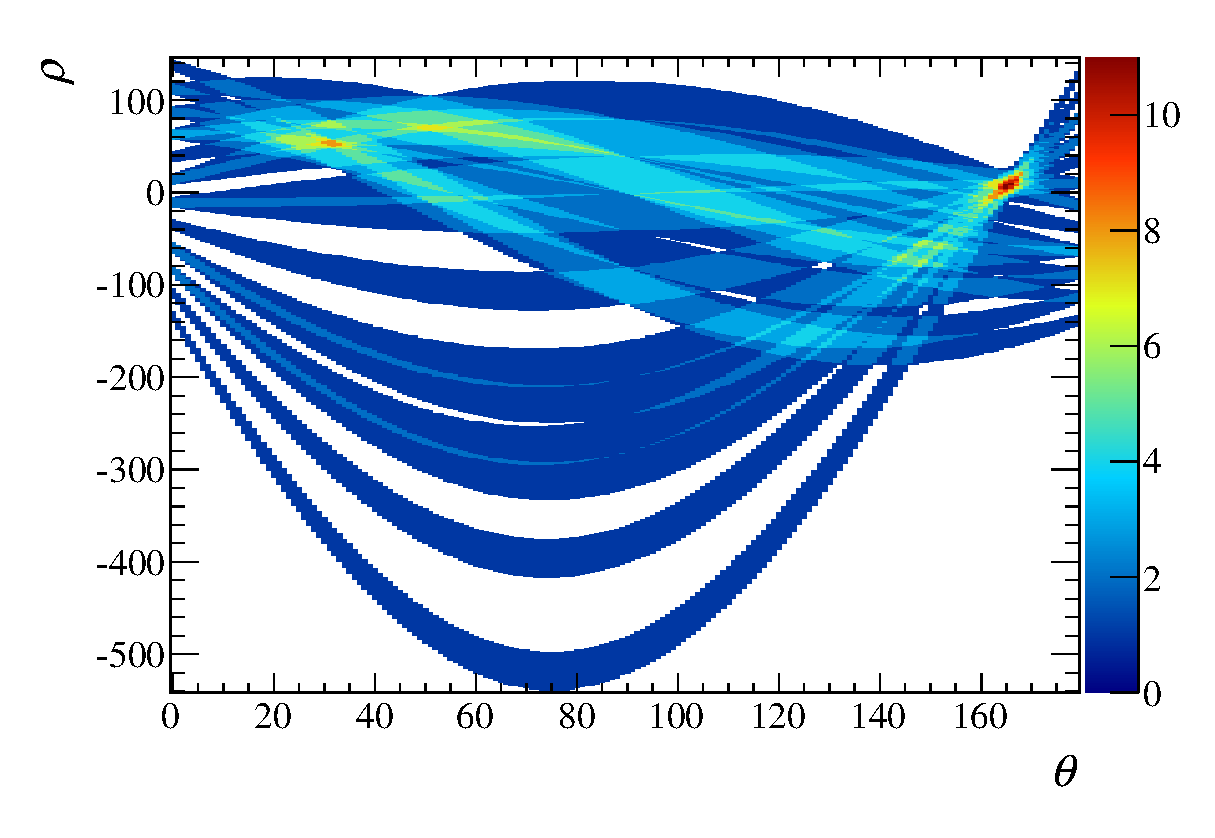
\includegraphics[width=10cm]{images/ecal_hough_transform/FullParameterSpace_3StateInteraction.eps}
  \caption{The full parameter space of the 2D cluster shown in Fig.~\ref{fig:3StateInteractionNoReconstruction}.}
  \label{fig:FullParameterSpace3StateInteraction}
\end{figure}


\subsection{Parameter space analysis}
\label{subsec:ParameterSpaceAnalysis}
The full parameter space can look arbitarily complicated. However, it contains a vast amount of trajectory related information about the cluster.  Every $\theta-\rho$ bin of the parameter space describes a 2D track and the content value of said bin describes how many 2D ECal hits the track passes through.  As described in section~\ref{sec:ECalApplicationHoughTransform}, a particles trajectory should be straight in the ECal which means that the particles path should be revealed by finding the most hits arranged in a line.  This hit arrangement can be found by finding the bin in the full parameter space with the highest value.  The track candidate parameters can the be found by fetching the ($\theta$,$\rho$) coordinate of the found bin.
\newline
While the preferred bin can reveal how many hits the track candidate passed through, it contains no information about which hits were contributors.  However, this full parameter space was generated by summing the $N$ parameter spaces discussed in section~\ref{subsec:ParameterSpaceGeneration}.  So, the contributing hits can be readily found by looking at the same ($\theta$,$\rho$) bin in each of the $N$ parameter spaces and recording which have a non-zero value.  We now have the track candidate's parameters and its contributing hits which is enough to describe the 2D trajectory.
\newline
A new search now needs to begin to find any other track candidates.  However, repeating the same search of the full parameter space will return the track candidate that has already been found.  To find the next track candidate, the presence of the previous track candidate must be removed.  So, a reduced parameter space must be generated. The previous step found which of the $N$ parameter lines contributed to the previous track candidate.  So, this new parameter space can be formed by subtracting the contributing parameter lines from the full space.  An example of this is shown in Fig.~\ref{fig:ReducedParameterSpace3StateInteraction} where the reduced parameter space was formed by subtracting the contributing parameter lines to the highest bin in Fig.~\ref{fig:FullParameterSpace3StateInteraction}.  The next track candidate can then be found by searching for the highest content bin of this reduced parameter space and said bin's contributing parameter lines. 
\newline
This process can be repeated until some threshold is reached.  This threshold is nominally set by demanding that at least three hits are required to form a track candidate.
\begin{figure}
  \centering
  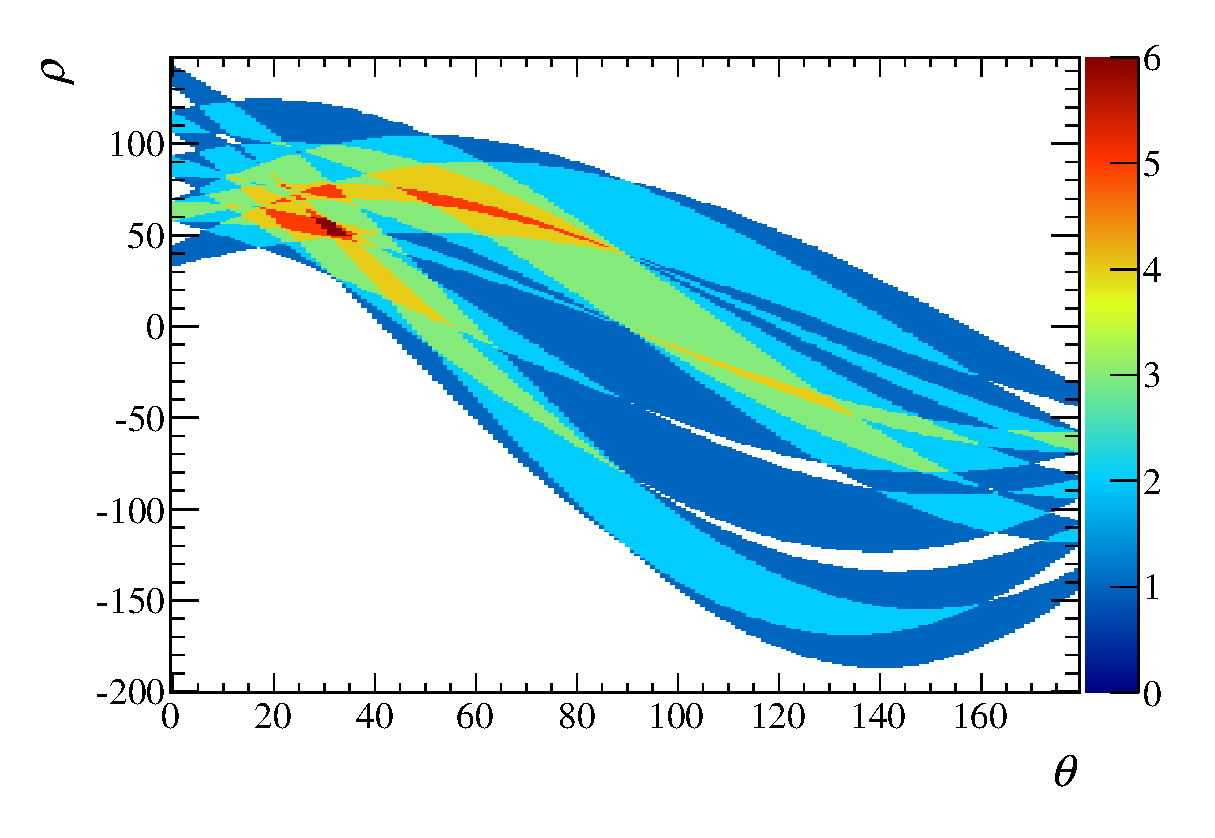
\includegraphics[width=10cm]{images/ecal_hough_transform/ReducedParameterSpace_3StateInteraction.eps}
  \caption{The reduced parameter space of the 2D cluster shown in Fig.~\ref{fig:3StateInteractionNoReconstruction}.}
  \label{fig:ReducedParameterSpace3StateInteraction}
\end{figure}


\subsection{3D track reconstruction}
\label{subsec:3DHoughTrackReconstruction}
Section~\ref{subsec:ParameterSpaceAnalysis} describes the track reconstruction of a 2D ECal cluster.  However, a 3D cluster consists of two sets of 2D clusters.  So, the process described in section~\ref{subsec:ParameterSpaceAnalysis} must be performed on each of the 2D clusters.  The result of this process is two sets of 2D tracks.  To form full 3D tracks, the tracks from each view must now be matched together.  This is acheived by making every pairwise comparison of the tracks from each view to find the pair which are most similar to each other.  After such a pair is found, the tracks are removed from the pool and the process is repeated to find the next pair until either no tracks are left or one 2D tracks are left.  In the latter case the single 2D track is discarded. Every pairwise combination of tracks is used to form a likelihood $\mathcal{L}$.  The pair which produces the highest $\mathcal{L}$ is declared the best match and removed from the pool.  Three pieces of information about the matching pair are used to calculate $\mathcal{L}$, all of which make use of probability density distributions generated using beam Monte Carlo.  
\newline
As should be expected, a vertex with one visible track will have different characteristics to a vertex with three visible tracks.  So, to maximise the ability of the matcher, a different set of probability density distributions are used for the 1, 2 and 3 track cases.  If the number of tracks in each view is not identical, the higher number of tracks is used to find the correct probability density distributions.  Seperately, due to their geometrical differences, the reconstructed shape of vertices in the DS ECal will differ to those in the barrel ECals.  This leads to a separate set of probability density distributions for the barrel and DS ECal modules.
\newline
The first input to the likelihood is the ratio of the total deposited charge on each track $Q_{\textrm{ratio}}$.  The denominator is taken as the track which comes from the view with the most hits.  Generally speaking, a particle propagating through an ECal module should deposit a similar amount of charge in each of the two views.  So, $Q_{\textrm{ratio}}$ should have a value close to 1 if the two 2D tracks are created by the same particle.  An example of the $Q_{\textrm{ratio}}$ distribution is shown in Fig.~\ref{fig:3DMatchingBarrel2TrackQRatioSeparation}, taken from beam Monte Carlo in the barrel ECals for cases where the maximum number of tracks found in a given view is 2.  In Fig.~\ref{fig:3DMatchingBarrel2TrackQRatioSeparation}, correctly matched (in blue) shows the $Q_{\textrm{ratio}}$ distribution for matching pairs which come from the same particle and incorrectly matched (in red) shows the the $Q_{\textrm{ratio}}$ distribution for matching pairs which were created by different particles.  As Fig.~\ref{fig:3DMatchingBarrel2TrackQRatioSeparation} shows, $Q_{\textrm{ratio}}$ well separates the two cases.  To generate a probability density distribution for $Q_{\textrm{ratio}}$, the two distributions shown in Fig.~\ref{fig:3DMatchingBarrel2TrackQRatioSeparation} are used, but without applying any normalisation.  By comparing the bins of each distribution, the probability for correctly matching two tracks in a given bin $p_{i}$ can be formed by
\begin{equation}
  p_i = \frac{s_i}{s_i + b_i}
  \label{eq:BinProbabilityPDF},
\end{equation}
where $s_i$ is the number of correctly matched tracks in bin $i$ and $b_i$ is the number of incorrectly matched tracks in bin $i$.  A discreet probability density distribution for $Q_{\textrm{ratio}}$ can then be formed by calculating $p_i$ for every bin.  The discreet probability density distribution is then interpolated with splines to create the final probability distribution.  An example of this for the two track, barrel case is shown in Fig.~\ref{fig:3DMatchingBarrel2TrackQRatioPDF}.  When a matching candidate pair is being considered, the value of $Q_{\textrm{ratio}}$ is calculated and used in the spline to retrieve $\mathcal{L}_{Q_{\textrm{ratio}}}$.
\begin{figure}
  \centering
  \parbox{7cm}{
    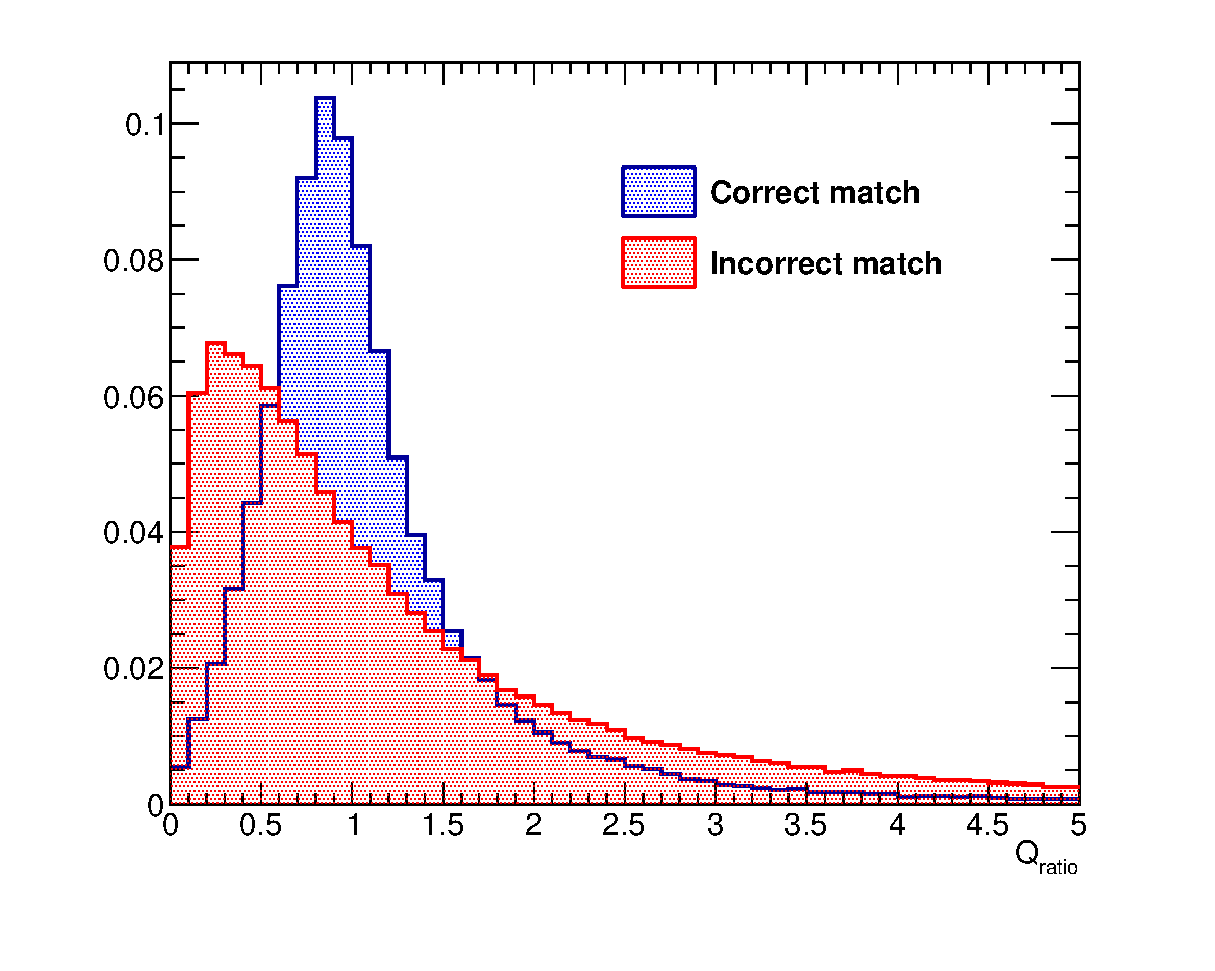
\includegraphics[width=7cm]{images/hough_3d_matching/3DMatching_Barrel_2Track_QRatio_Separation.eps}
    \caption{$Q_{\textrm{ratio}}$ distribution in the barrel ECal for the two track case.  The blue distribution refers to matching pairs which were matched to the same true particle.  Both distributions are unit normalised.}
    \label{fig:3DMatchingBarrel2TrackQRatioSeparation}}
    \qquad
    \begin{minipage}{7cm}
      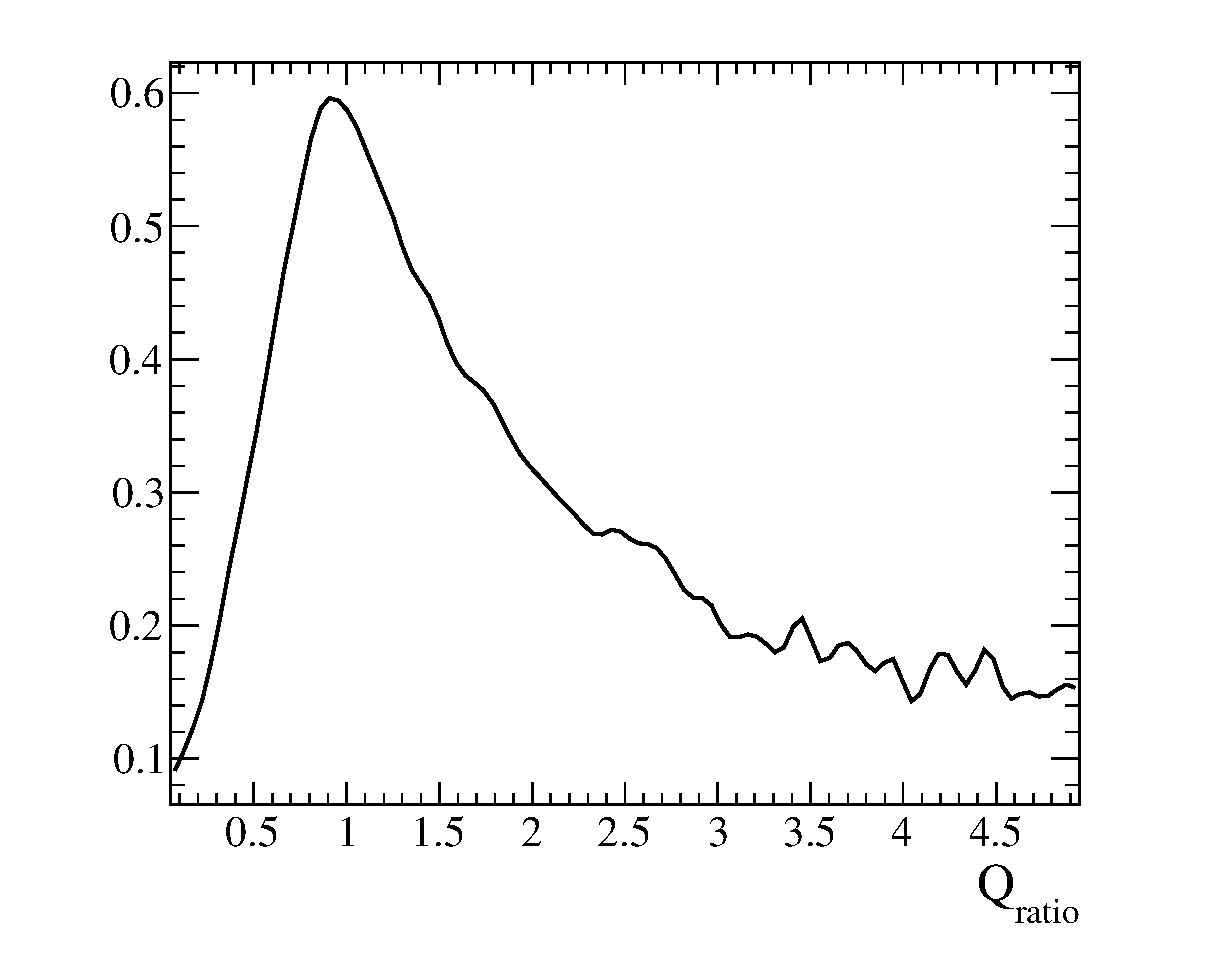
\includegraphics[width=7cm]{images/hough_3d_matching/3DMatching_Barrel_2Track_QRatio_PDF.eps}
      \caption{$Q_{\textrm{ratio}}$ probability density distribution in the barrel ECal for the two track case.}
      \label{fig:3DMatchingBarrel2TrackQRatioPDF}
    \end{minipage}
\end{figure}
\newline
The second input to the likelihood, called $\Delta_{\textrm{layer, first}}$, is the difference in the starting layer of each 2D track which forms the matching candidate pair, where starting layer refers to the layer closest to the ND280 tracker.  For 2D tracks which should be matched together, $\Delta_{\textrm{layer, first}}$ should be 1.  The separation ability of this variable for the two track, barrel is shown in Fig.~\ref{fig:3DMatchingBarrel2TrackDFLSeparation}.  The discreet probability density function was created using eqn.~\ref{eq:BinProbabilityPDF}.  It was not necessary to interpolate using splines as $\Delta_{\textrm{layer, first}}$ is itself discreet.  The probability density function for $\Delta_{\textrm{layer, first}}$ is shown in Fig.~\ref{fig:3DMatchingBarrel2TrackDFLPDF} for the two track, barrel case.  For each matching candidate pair, the value of $\Delta{\textrm{layer, first}}$ is calculated and the corresponding $\mathcal{L}_{\Delta_{\textrm{layer, first}}}$ is retrieved from the probability density function.
\begin{figure}
  \centering
  \parbox{7cm}{
    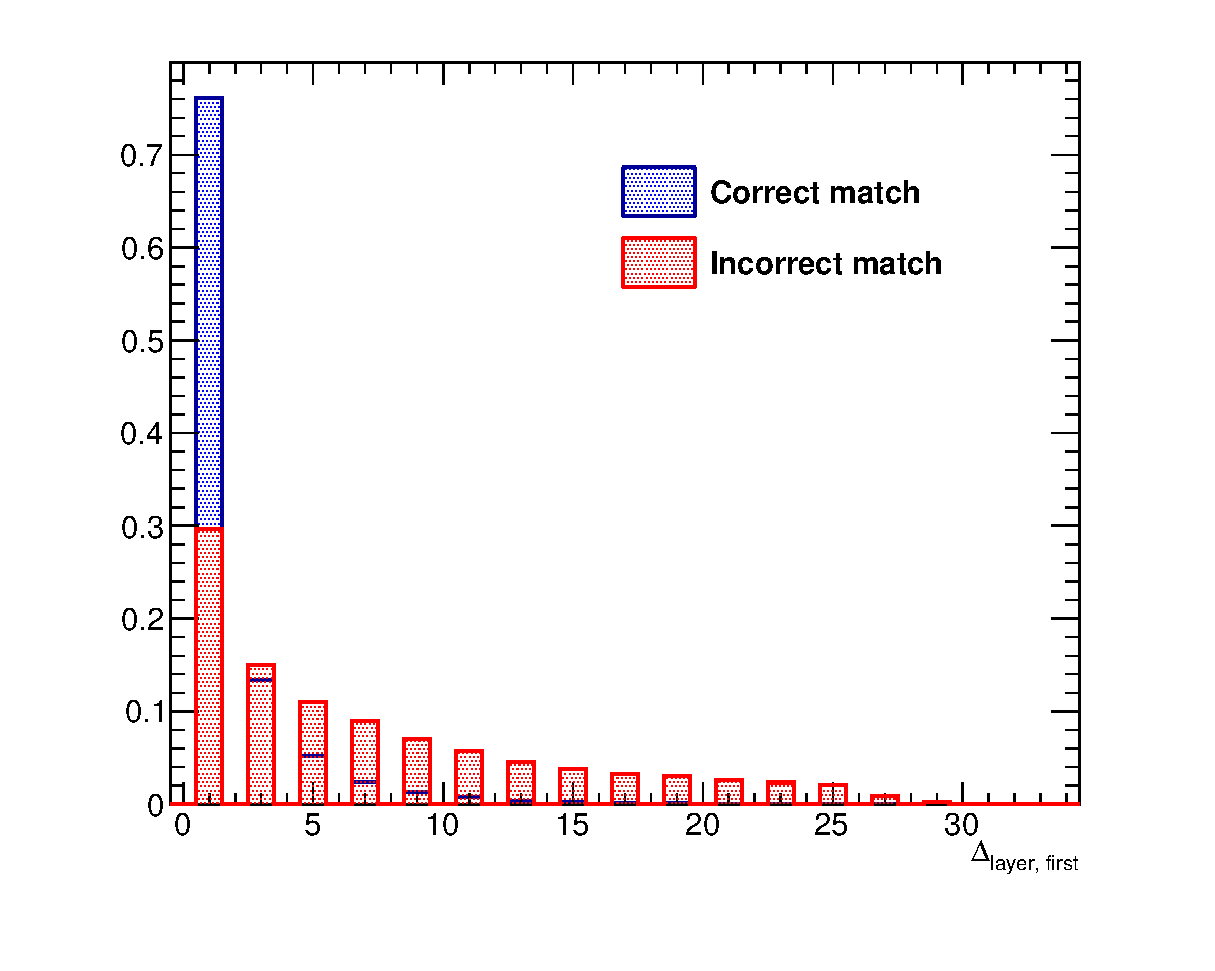
\includegraphics[width=7cm]{images/hough_3d_matching/3DMatching_Barrel_2Track_DFL_Separation.eps}
    \caption{$\Delta_{\textrm{layer, first}}$ distribution in the barrel ECal for the two track case.  The blue distribution refers to matching pairs which were matched to the same true particle.  Both distributions are unit normalised.}
    \label{fig:3DMatchingBarrel2TrackDFLSeparation}}
    \qquad
    \begin{minipage}{7cm}
      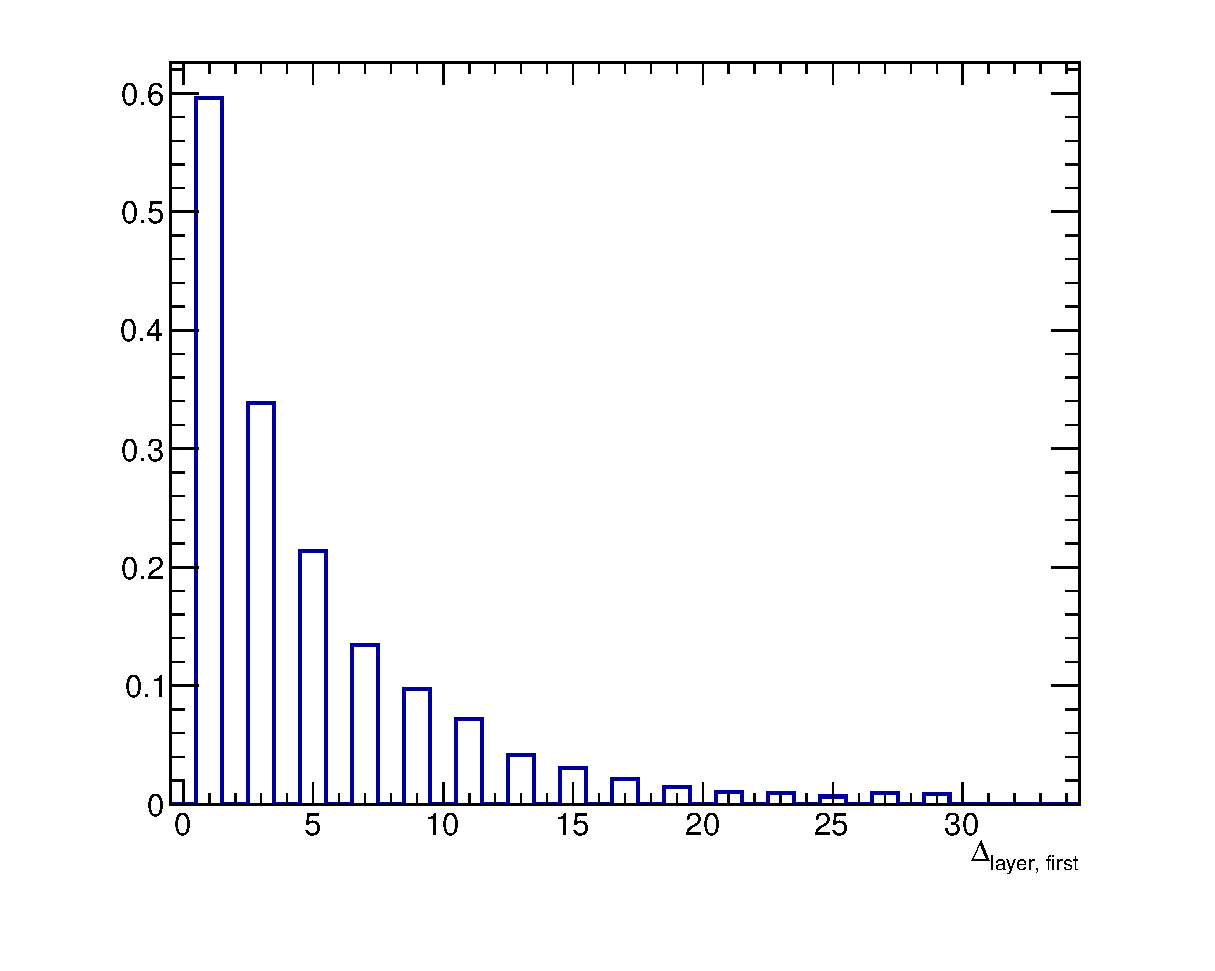
\includegraphics[width=7cm]{images/hough_3d_matching/3DMatching_Barrel_2Track_DFL_PDF.eps}
      \caption{$\Delta_{\textrm{layer,first}}$ probability density distribution in the barrel ECal for the two track case.}
      \label{fig:3DMatchingBarrel2TrackDFLPDF}
    \end{minipage}
\end{figure}
\newline
The third and final input to the likelihood, called $\Delta_{\textrm{layer, last}}$, is the differnce in the ending layer of each 2D track which forms the matching cadidate pair, where the ending layer refers to the layer furthest from the ND280 tracker.  Functionally, how this function is used is essentially identical to $\Delta_{\textrm{layer, last}}$ so it will not be described in detail.  The separation ability of this variable and its corresponding probabilty density function for the two track, barrel case are shwon in Fig.~\ref{fig:3DMatchingBarrel2TrackDLLSeparation} and Fig.~\ref{fig:3DMatchingBarrel2TrackDLLPDF} respectively.
\begin{figure}
  \centering
  \parbox{7cm}{
    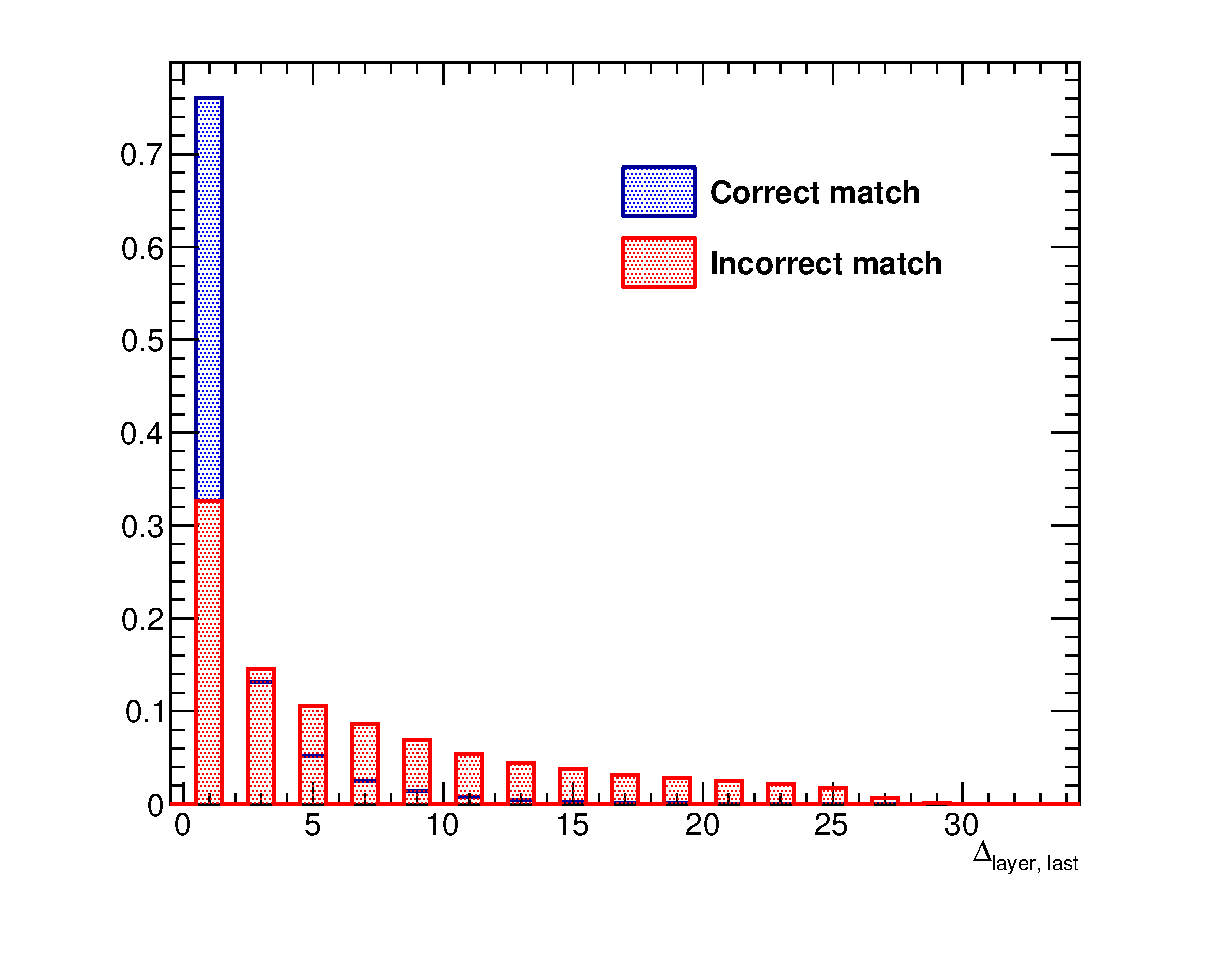
\includegraphics[width=7cm]{images/hough_3d_matching/3DMatching_Barrel_2Track_DLL_Separation.eps}
    \caption{$\Delta_{\textrm{layer, last}}$ distribution in the barrel ECal for the two track case.  The blue distribution refers to matching pairs which were matched to the same true particle.  Both distributions are unit normalised.}
    \label{fig:3DMatchingBarrel2TrackDLLSeparation}}
    \qquad
    \begin{minipage}{7cm}
      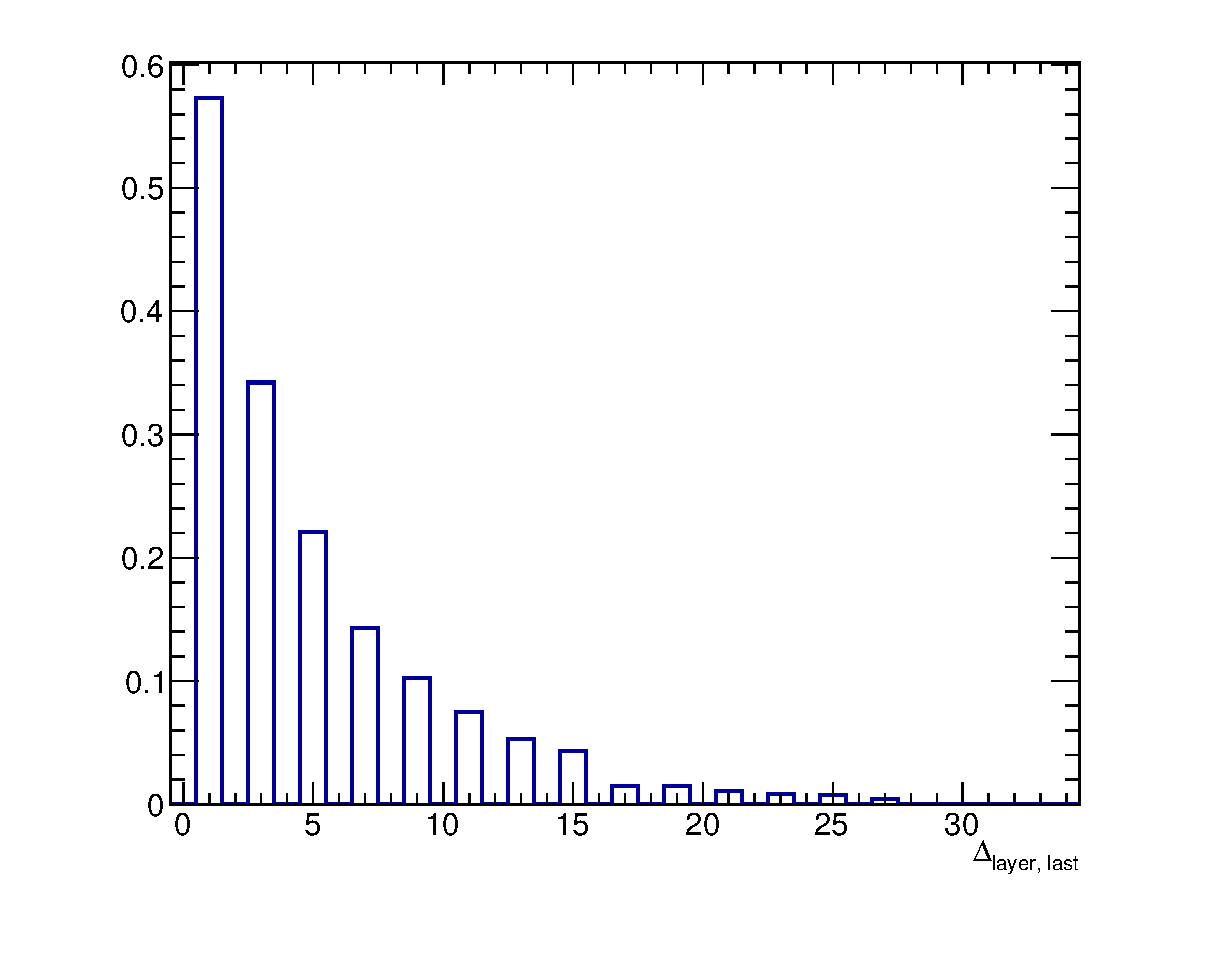
\includegraphics[width=7cm]{images/hough_3d_matching/3DMatching_Barrel_2Track_DLL_PDF.eps}
      \caption{$\Delta_{\textrm{layer,last}}$ probability density distribution in the barrel ECal for the two track case.}
      \label{fig:3DMatchingBarrel2TrackDLLPDF}
    \end{minipage}
\end{figure}
\newline
The matching likelihood, $\mathcal{L}$ for a matching candidate pair is then
\begin{equation}
  \mathcal{L} = \mathcal{L}_{Q_{\textrm{ratio}}} \times \mathcal{L}_{\Delta_{\textrm{layer, first}}} \times \mathcal{L}_{\Delta_{\textrm{layer, last}}}.
\end{equation}
As described above, $\mathcal{L}$ is calculated for every matching candidate pair and the pair which maximise $\mathcal{L}$ is selected as a match and removed from the pool.  The process is then repeated until no more matches can be made.
\newline
3D tracks have now been formed, but the associated directions and positions of those tracks still need to be calculated.  The track fitting process for the newly formed 3D tracks is very similar to that described in section~\ref{subsec:ECal3DHitReconstruction}.  The tracks are briefly separated into their constituent 2D views and a charge-weighted average position of each layer is calculated using the track's constituent hits.  Then, the hits in the opposing view are used to estimate the 3rd coordinate of a given layer using a least-squares fit.  After all of the coordinates have been estimated, a full 3D least-squares fit of the positions in each layer is performed to estimate the 3D track's direction and position in that ECal layer.

\subsection{Track pairwise crossing reconstruction}
\label{subsec:TrackCrossingReconstruction}
The final step of the reconstruction is to estimate where each of the 3D track's paths cross.  As each track is reconstructed as a straight line in 3D, the final step is fairly simple.  Using the track direction and position information calculated at the end of section~\ref{subsec:3DHoughTrackReconstruction}, the position at closest approach for every pairwise combination of 3D tracks is calulated analytically.  The distance of closest approach is also calculated.  Six hits, the closest three from each 3D track, are then associated to the pairwise crossing. 

\section{Output of the reconstruction}
The reconstruction is run over every 3D cluster found in the ECal.  By applying the steps outlined above, for each 3D cluster the following output is given:
\begin{itemize}
  \item A set of 3D tracks
  \item The pairwise crossings of all 3D tracks found in the cluster
\end{itemize}
Note that no vertex formation beyond the pairwise crossings is calculated at this stage, nor is any analysis of the 3D tracks performed.  While this may seem like an oversight of the reconstruction, this approach was decided as no assumptions are made about what the tracks/crossings represent at this point, making the output more generic.  Any analysis which wants to make use of the reconstruction is given enough information to apply more targeted reconstruction downstream. 


%
%To build the probability density distributions, the output of the 2D reconstruction was used to form every possible matching pair (as described above) and the results were separated into two distinct catagories: correctly matched and incorrectly matched.
\section{Validation of the reconstruction}
\label{sec:ReconstructionValidation}
Someone do this plz 
